\section{RESULTS}\label{sec:4experiment}
In this section, we detail the evaluation results for our system.

\subsection{Evaluation of Subcomponents}
We focus on the detection accuracy about five events, that are body posture, the body rollover, the hand position, the micro body movement and the acoustic events.
%, the classification of micro body movement

\subsubsection{Sleep Posture Classification Performance}
\label{subsub:bodyposture}

We first test the overall classification performance of different body postures. The ground truth of body postures are recorded by the cameras. To avoid biases in evaluation, and to assess the generalization performance of our approach, we consider a cross-validation scheme where all data from a single participant is used for training and data from the remaining $14$ participants is used for testing. The motivation for using data from a single user as training data is to highlight the capability of \systemname to accurately characterize body posture with very little training data, while at the same time being able to generalize across users.  The final performance is then calculated as the averaged accuracy across the 15 folds; as shown in Fig.~\ref{fig:posture_zhu} and Table \ref{tab:posture}. We can observe that the posture detection accuracy is consistently high across all users, and does not show major variations across users. This good performance benefits from the distinct characteristics of arm position under different sleeping postures. Compared to results reported for SleepMonitor~\cite{sleepmonitor}, \systemname consistently improves performance which is mainly due to the template-based classifier that we use to verify classifications of the prone and supine states. In particular, \systemname achieves around $5$ percentage units higher performance on the prone state than SleepMonitor and overall has a lower false positive rate. In terms of errors, due to angular characteristics of acceleration being similar between the supine posture with hand putting on the head and the left-lateral posture, a small amount of the supine postures are classified as left lateral. From the results we can also observe that the total amount of the prone posture is smaller than the number of other postures, which suggests that people are not accustomed to sleep in this position, because it is neither healthy nor comfortable.%

\begin{figure}
	\centering
	\begin{minipage}{.5\textwidth}
	 \centering
	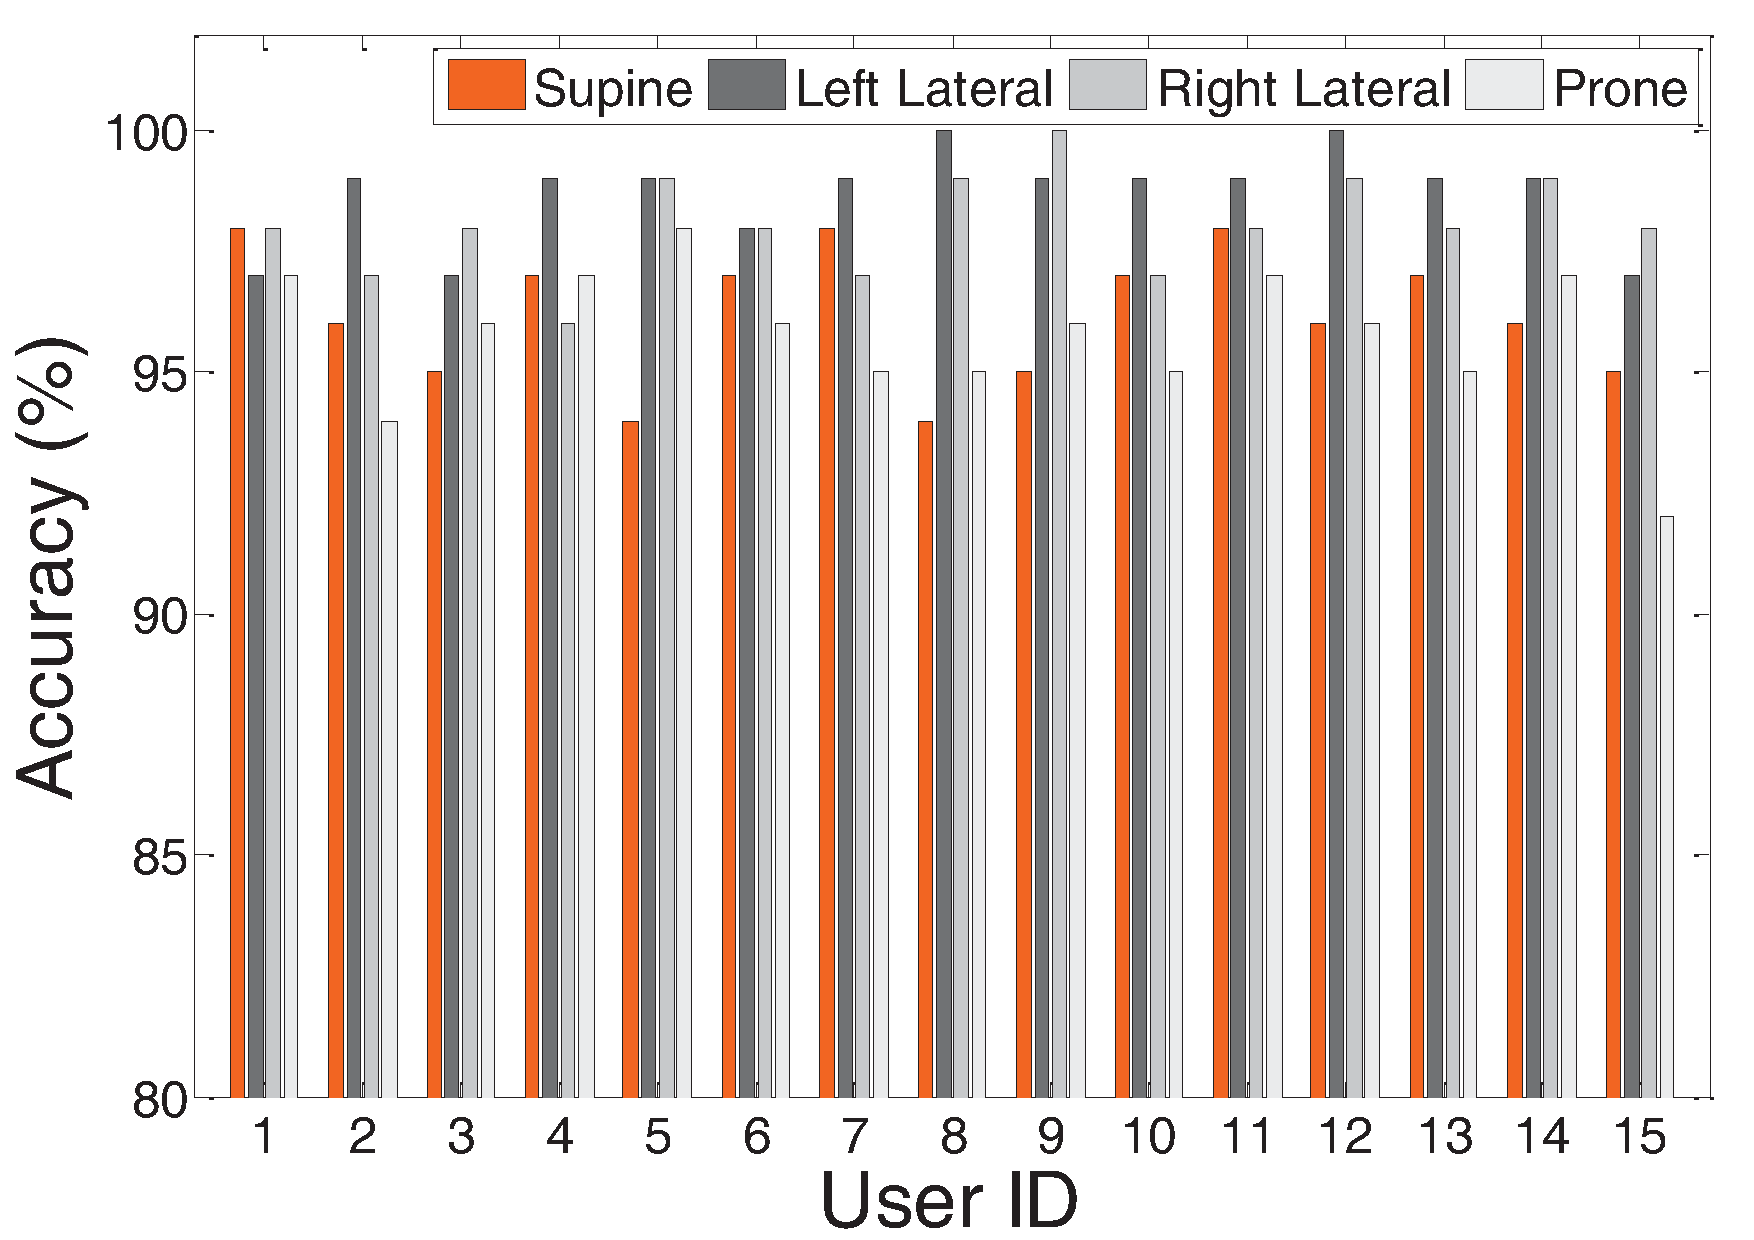
\includegraphics[width=0.95\linewidth]{Figures/posture_zhu.pdf}
	\caption{Detection accuracy of body postures.}\label{fig:posture_zhu}
	\end{minipage}%
	\begin{minipage}{.5\textwidth}
			\centering
		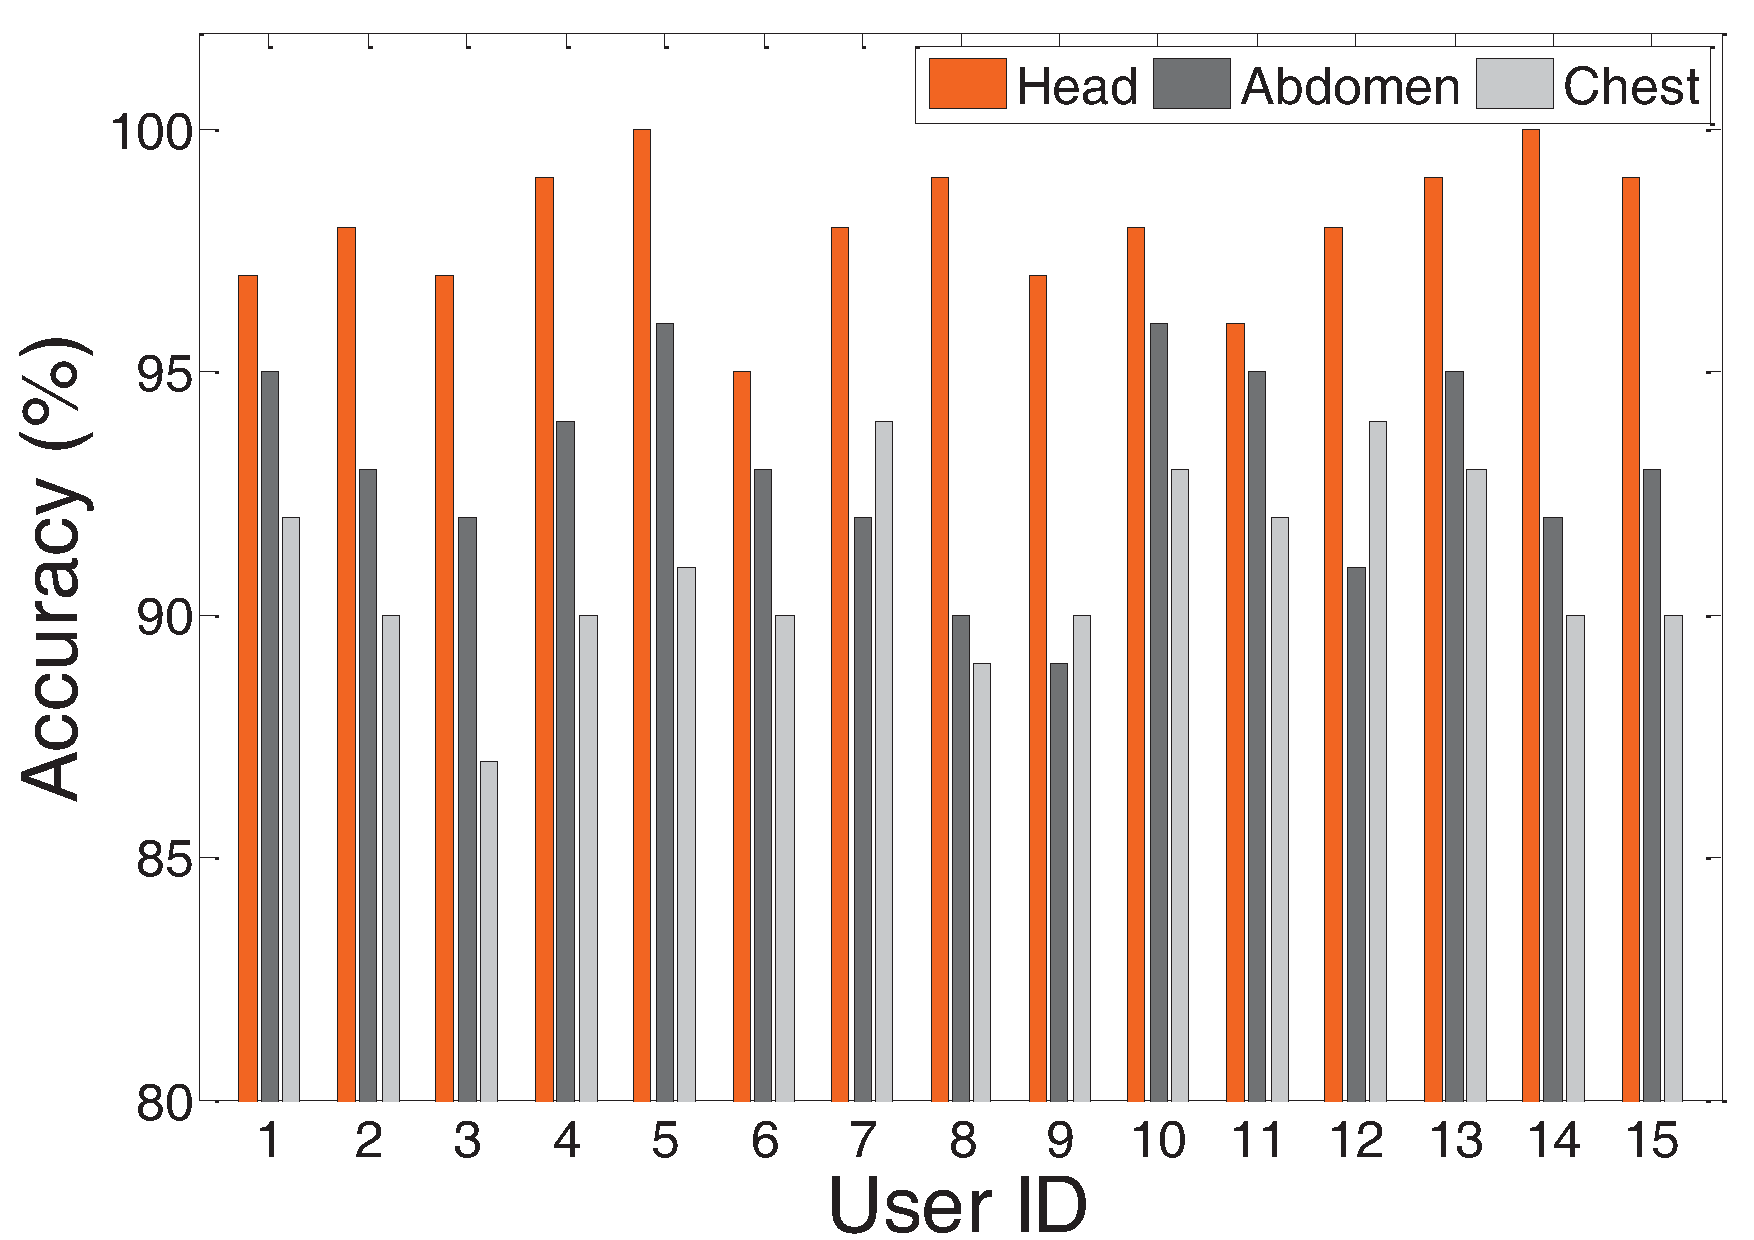
\includegraphics[width=0.95\linewidth]{Figures/handposition_zhu.pdf}
		\caption{Identification accuracy of hand positions.}\label{fig:hand_zhu}
	\end{minipage}
\end{figure}

\begin{table}[!t]\footnotesize
%	\tabcolsep1pt
	\centering  % ������
	%\renewcommand\arraystretch{0.277}
	%\caption{The confusion matrix of body posture classification.}\label{tab:posture}
	%\noindent\makebox{%
	%\begin{tabular}{1\textwidth}{ c | c | c | c | c | c | c}
	\renewcommand\arraystretch{0.3}
	\caption{The confusion matrix of body posture classification.}\label{tab:posture}
	\begin{tabular}{c| c | c | c | c | c | c}
		\cline{1-7}
		&\multicolumn{1}{ c|}{ }
		& \multicolumn{4}{ c|}{ }\\
		\multirow{2}*{}
		&\multicolumn{1}{c|}{\multirow{2}*{{Result}}}
		&\multicolumn{4}{c|}{{Prediction}}
		& \multirow{4}*{{Recall}} \\
		%&\multicolumn{5}{ c |}{\textbf{\small Prediction}} \\
		% & \multicolumn{5}{ c |}{ } \\
		\cline{3-6}
		& & & & & \\
		\multicolumn{1}{c|}{{}}
		&  \multicolumn{1}{c|}{{}}
		&  \multicolumn{1}{c|}{{Supine}}
		&  \multicolumn{1}{c|}{{Left Lateral}}
		&  \multicolumn{1}{c|}{{Right Lateral}}
		&  \multicolumn{1}{c|}{{Prone}}   \\
		& & & & & \\
		\cline{1-7}
		& & & & & \\
		\multirow{5}{*}{\begin{sideways}{{Groundtruth}}\end{sideways}}
		&   {Supine}   & {\bf{{1182}}}    &   $25$      &   $4$      &   $9$    &   {96.7\%}\\
		& & & & & \\
		\cline{2-7}
		& & & & & \\
		&   {Left Lateral}   &   $6$      &   {\bf{{1292}}}     &   $0$      &   $0$   &   {99.5\%} \\
		& & & & & \\
		\cline{2-7}
		& & & & & \\
		&   {Right Lateral}   &   $7$      &   $0$      &  {\bf{{1275}}}      &   $12$  &   {98.5\%}  \\
		& & & & & \\
		\cline{2-7}
		& & & & & \\
		&   {Prone}   &   $19$      &   $2$      &   $3$      &   {\bf{{567}}}   &   {95.9\%} \\
		& & & & & \\
		\cline{1-7}
		& & & & & \\
		&   {Precision}    &   {97.3 \%}   &   {98.0\%}   &   {99.5\%}   &   {96.4\%}    \\
		& & & & & \\
		\cline{1-7}
	\end{tabular}
\end{table}

%To have a deep evaluation about the sleep posture detection, we randomly choose one user to train the classifier. Then we calculate the detection precision and recall across postures. \textcolor{blue}} The values in blocks are the corresponding numbers of four sleep postures from 14 test users.

%In conclude, Table \ref{tab:posture} shows the outstanding detection performance.



\subsubsection{Performance of body rollover counting}
To verify the efficiency of body rollover detection algorithm, we compare each user's  body rollover events detected by {\systemname}
against the data labeled by watching the video. The performance is showed in Table \ref{tab:rollver}. We can see that User 3, User 4 and
User 13 have an unusually high number of rollovers. For User 3 and User 4, they have difficulty in falling asleep due to the sleep
disorder. User 13 needs to rollover frequently because of  his loudly snoring. As we demonstrate in Sec.~\ref{sec:user_survey}, these
participants also suffered from poor sleep quality and hence indicate how the information extracted by \systemname can support the
detection of sleep problems. For all the 15 users, the detection accuracies are all very high, and the lowest one is still 87\%. Thus
{\systemname} can accurately distinguish the large hand movement from the body rollover in bed. Moreover, detecting errors in body rollover
events will not have a significant impact on our end result, because the division of  sleep stages is a comprehensive consideration of all
the detected features in each stage, such as micro body movement and acoustic events.

\begin{table}[!thbp]\footnotesize
  %\centering  % ������
 % \tabcolsep 1pt
  %\arrayrulewidth1pt
  \caption{Detection accuracy of body rollover.}\label{tab:rollver}
   \renewcommand\arraystretch{1}{\multirowsetup}{\centering}
        \begin{tabular}{cccccccccccccccc}
        \toprule
         \textbf{Testing User ID}    & 1& 2  & 3& 4& 5& 6& 7& 8& 9& 10& 11& 12& 13& 14& 15\\
        \midrule
             {Labeled \#body rollover}  &231&204&442&397&198&101&196&164&193&208&131&205&342&149&156 \\
                 { Accuracy} &91\%& 94\% &88\%&93\%&96\%&94\%&87\%&90\% &93\% &94\% &92\% &94\% &89\% &90\% &95\%\\
        \bottomrule
 \end{tabular}
\end{table}

\subsubsection{Performance of hand position recognition}
To test the recognition performance of different hand positions, we consider the same cross-validation scheme used for body posture
detection, i.e., one user's data is used for training the classifier and the remaining 14 users' data as test data. The classifier for
detecting the hand movement trajectory is combined with the detection of periodic signals caused by respiration, then the hand position on
the chest (or abdomen or head) can be identified. \rt{In our dataset, 14\%, 36\% and 22\% of the time the hand in the supine posture during
sleep was placed on the head, abdomen, and chest respectively.} Fig.~\ref{fig:hand_zhu} illustrates the accuracy of hand position across 15
users. As we can see that with just one set of training data, the accuracies for different users are all higher than 87\%. Therefore, our
system can achieve a good identification accuracy for different hand positions. Moreover, we find that at least four out of fifteen
participants tend to put their hands on their heads; one participate unconsciously puts his hand on his chest which makes him have
nightmares. Those are all bad habits disrupting a good sleep.  {\systemname} can report such key findings to improve the users' sleep
qualities.


\subsubsection{Performance of micro body movement detection}

To assess the detection accuracy of micro body movements, we manually label the ground truth recorded by the camera during sleep, including
hand moving, arm raising, and body trembling. We also use the accelerometer embedded in the smartphone which placed on the bed to record
the occurrence of micro body movements, so as to avoid missing some movements such as trembling concealed by the duvet. For the
acceleration data collected by smartphone, we first smooth the acceleration along the three axes, calculate Root Sum Square (RSS) to merge
them, and obtain the first-order derivative of the merged acceleration. And then we use the threshold detection method to mark the
occurrence of motion. Since body trembling is the easiest to be covered, we only focus on such events. So we use smartphone to detect the
occurrence of events and the classification of the event is not performed. \rt{ Table~\ref{tab:micro_move} list the total number of three
micro body movements for each user over the testing period of 14 days, and Fig.~\ref{fig:micro_movement_zhu} reports the accuracy of
\systemname for detecting these micro body movements.} It shows that the accuracies for all users are very close, that is, there will be no
major changes between users. And from Fig. \ref{fig:micro_combine}, we find that even though the worst classification result belongs to the
hand movement, the average precision value and recall value still exceed 75\%. The averaged accuracies of arm raising and body trembling
are 93\% and 84\%, respectively. Because the training data volume for the hand movement and body trembling is small, so the performance can
be improved by setting each user a threshold by collecting a longer term's sleeping data. In addition, the purpose of  micro body movement
detection is to detect different sleep stages, and the hand movement usually appears in all sleep stages, thus the poor accuracy of hand
moving does not have a significant impact on the final result.


\begin{figure}
	\centering
	\begin{minipage}{.5\textwidth}
		 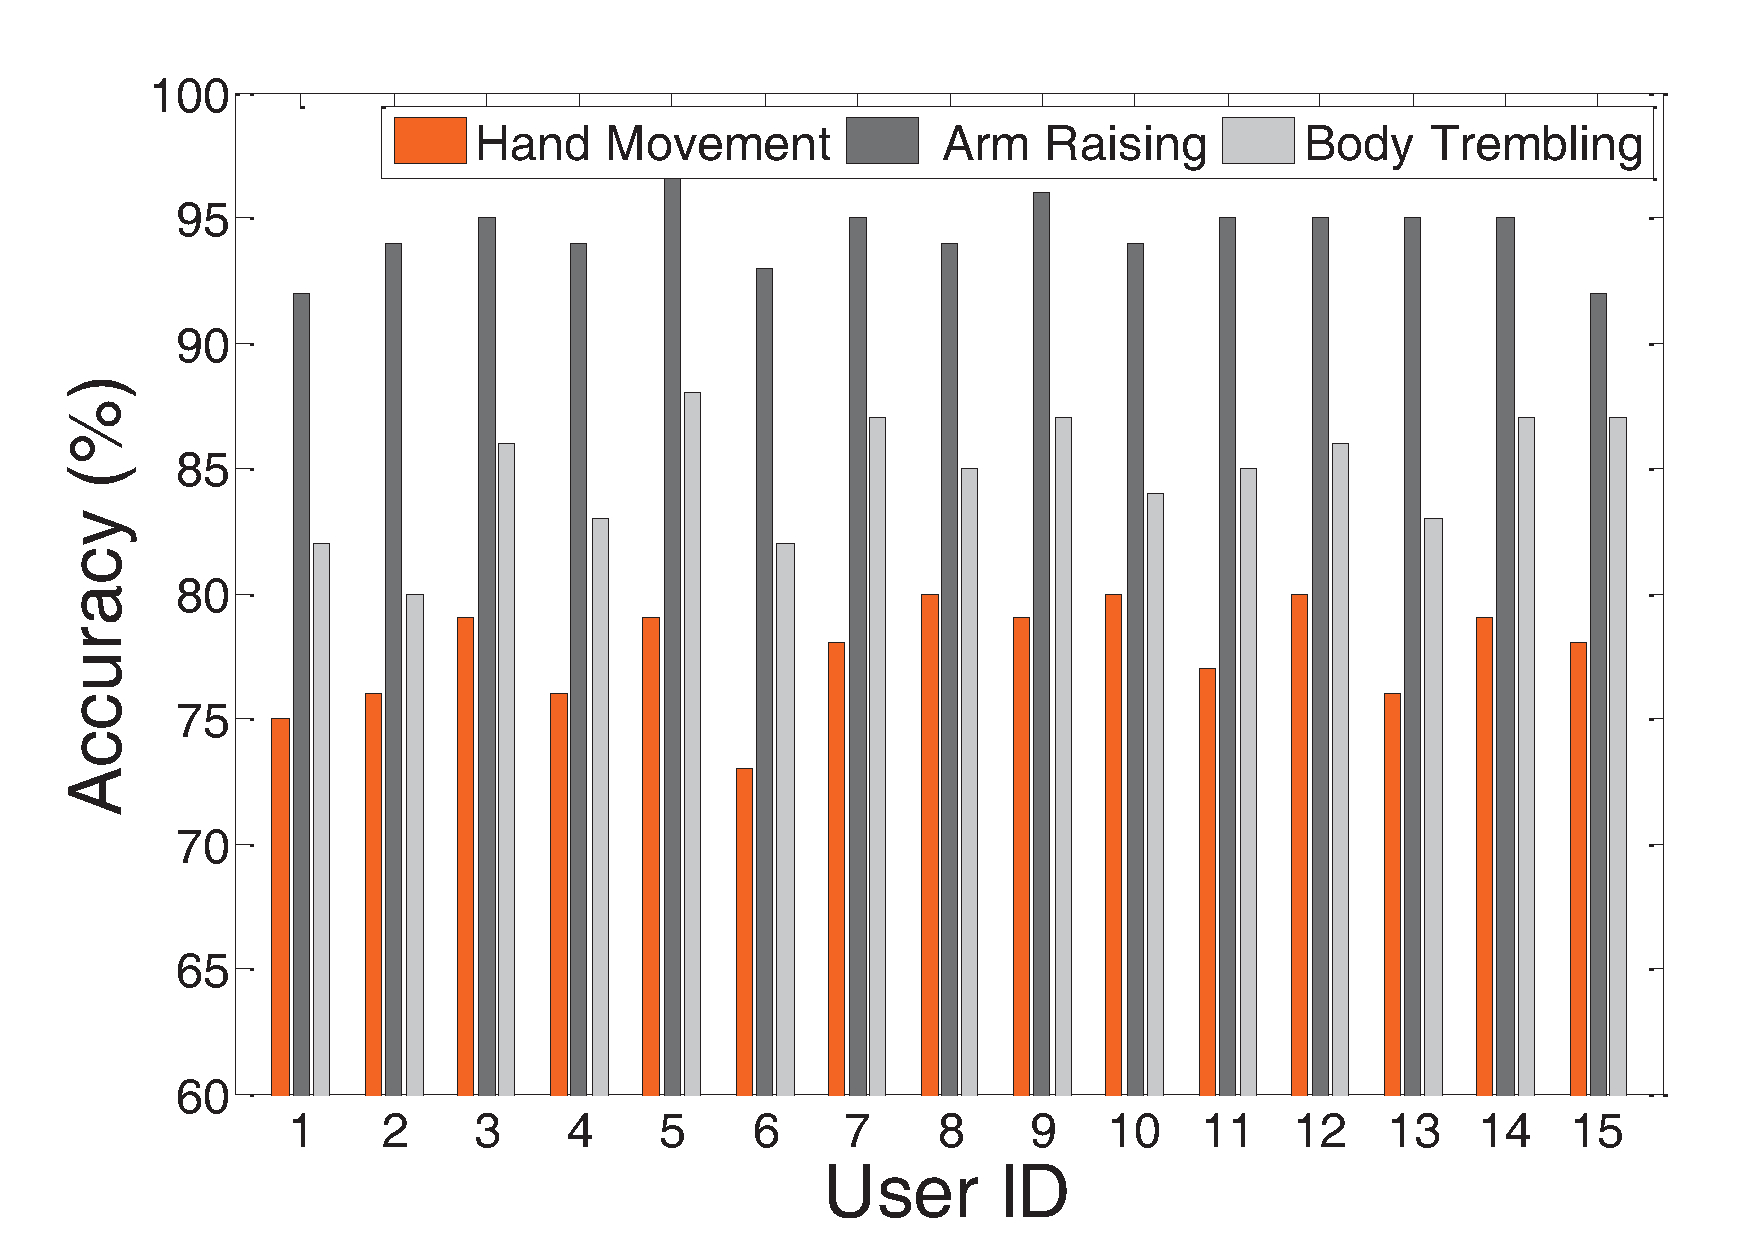
\includegraphics[width=1\textwidth]{Figures/micro_movement_zhu.pdf}
		\caption{Micro body movement detection accuracy.}\label{fig:micro_movement_zhu}	
	\end{minipage}%
	\begin{minipage}{.5\textwidth}
	 \centering
	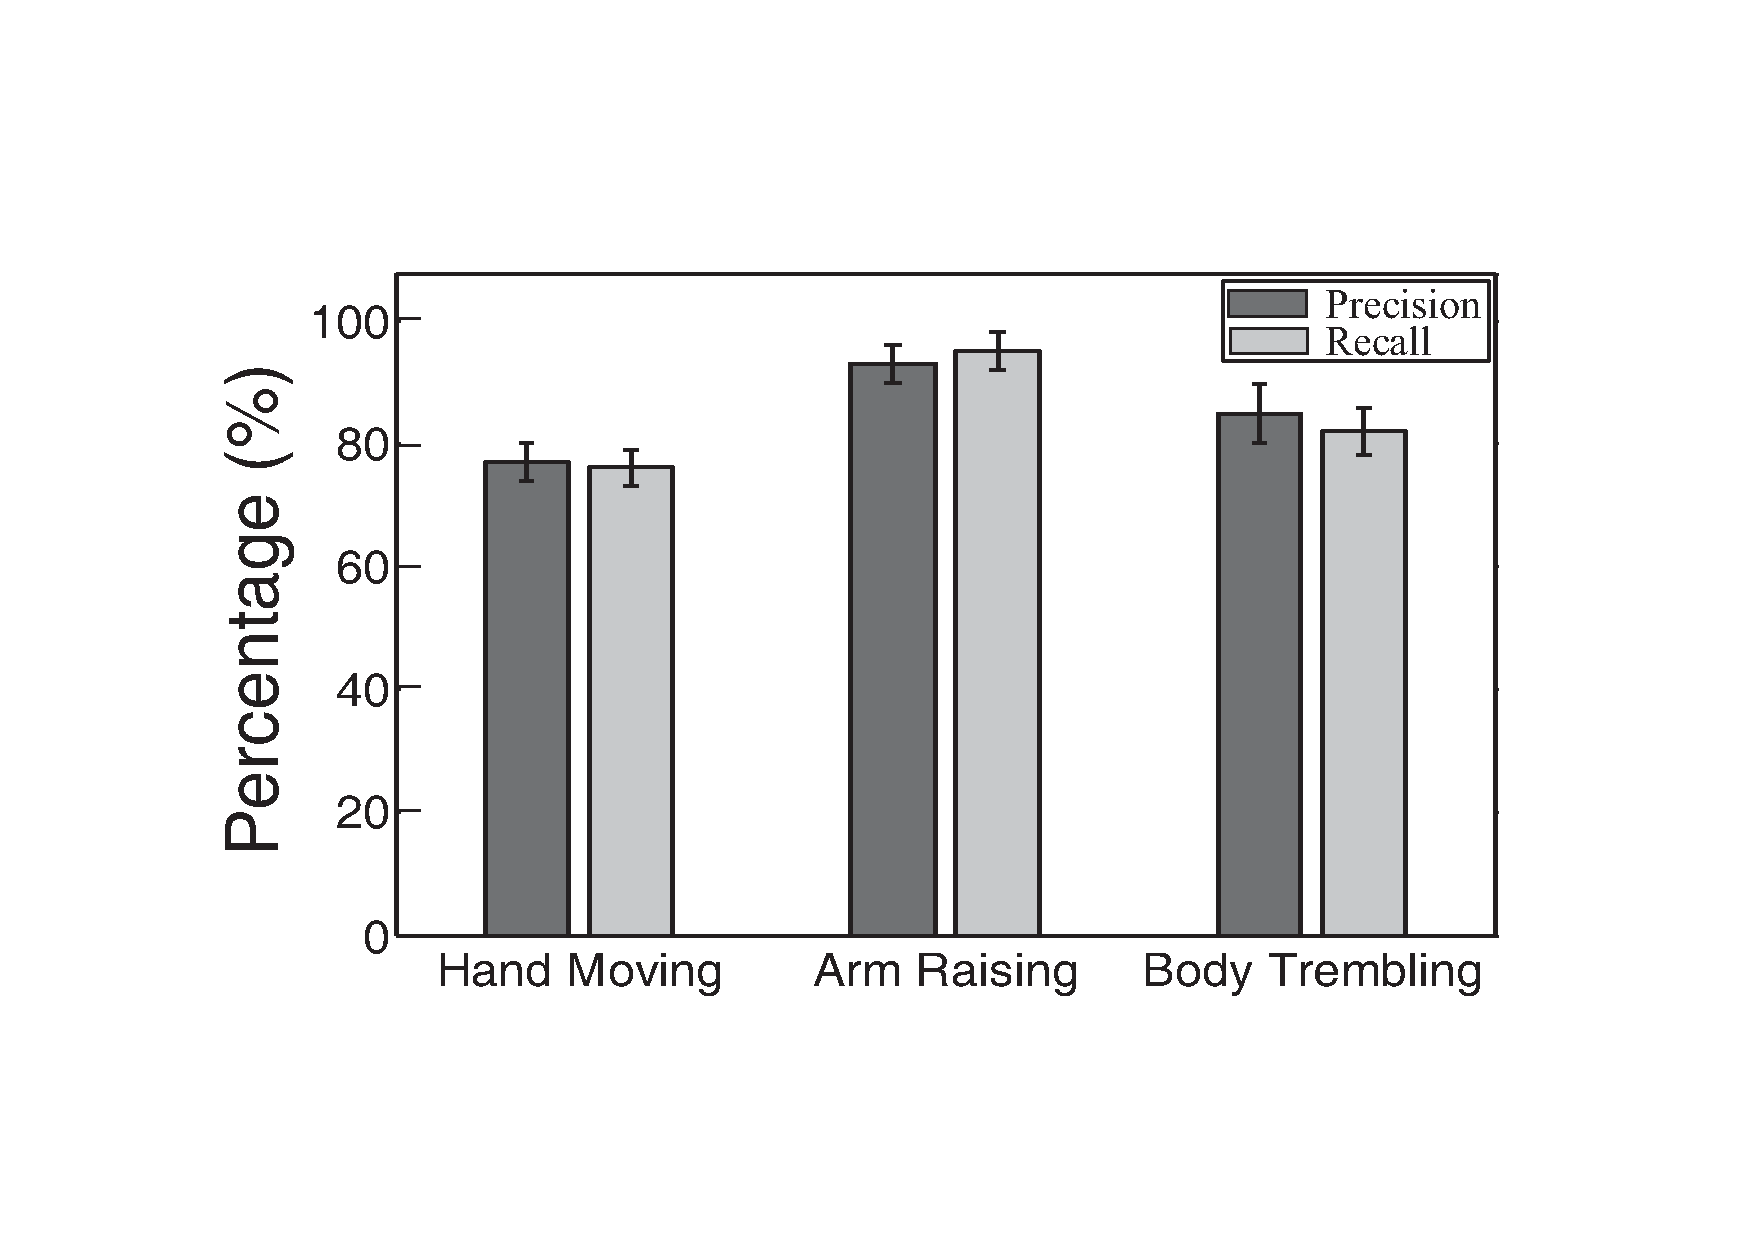
\includegraphics[width=1\textwidth]{Figures/micro_combine1.pdf}
	\caption{Precision and recall for micro body movement detection.}\label{fig:micro_combine}
	\end{minipage}
\end{figure}


\begin{table}[!t]\footnotesize
  %\centering  % ������
 % \tabcolsep 1pt
  %\arrayrulewidth1pt
  \caption{The number of micro body movements per user.}\label{tab:micro_move}
   \renewcommand\arraystretch{1}{\multirowsetup}{\centering}
        \begin{tabular}{lccccccccccccccc}
        \toprule
         \textbf{Testing User ID}    & 1& 2  & 3& 4& 5& 6& 7& 8& 9& 10& 11& 12& 13& 14& 15\\
        \midrule
            \rowcolor{Gray} {Labeled \#hand movement}  &52&49&67&55&58&55&59&56&61&53&57&55&60&59&62 \\
             { Labeled \#arm raising} &48&44&48&53&46&49&47&50&53&45&54&49&57&46&51\\
             \rowcolor{Gray} { Labeled \#body trembling} &28&32&25&29&34&25&20&30&24&26&27&35&24&22&25\\
        \bottomrule
 \end{tabular}
\end{table}


 \subsubsection{Performance of acoustic events detection}

To study the detection accuracies of different acoustic events, we compare the ground truth recorded by the camera with the detected results by our system. Table~\ref{tab:sound} shows the results across 15 participants. We can see that the precision for cough event is 88.9\%, which is slightly lower than for the other three event types. The reason is that different user's cough patterns are different, the pre-defined parameters in the detection model does not include all possible patterns. For example, some people have a fast and continuous pattern of coughing, while others have a slower intermittent pattern. In fact, we train these parameters, namely the "interval", "duration" and "frequency" of acoustic events, with only 120 sets of nighttime sound data. Those data come from 40 (21 males and 19 females) volunteers of different ages (from 15 to 60 years old) who are prone to snoring, coughing, or somniloquy at night. To further improve the detection accuracy, we can train particular parameters for different users. And we can further expand the training data to include more possible patterns, and can also make reasonable estimates of the possible patterns to refine the range of parameters and thus increase the accuracy.


\begin{table}[!t]\footnotesize
% \tabcolsep1pt
  \centering  % ������
 \renewcommand\arraystretch{0.3}
  \caption{The confusion matrix of acoustic events detection.}\label{tab:sound}
\begin{tabular}{c| c | c | c | c | c | c}
   \hline
   &\multicolumn{1}{ c|}{ }
   & \multicolumn{4}{ c|}{ }\\
   \multirow{2}*{}
&\multicolumn{1}{c|}{\multirow{2}*{{ Result}}}
&\multicolumn{4}{c|}{{ Prediction}}
& \multirow{4}*{{ Recall}} \\
    %&\multicolumn{5}{ c |}{\textbf{\small Prediction}} \\
   % & \multicolumn{5}{ c |}{ } \\
    \cline{3-6}
    & & & & & \\
    \multicolumn{1}{c|}{{}}
    &  \multicolumn{1}{c|}{{}}
    &  \multicolumn{1}{c|}{{ Snore}}
    &  \multicolumn{1}{c|}{{ Cough}}
    &  \multicolumn{1}{c|}{{ Somniloquy}}
    &  \multicolumn{1}{c|}{{ Other}}   \\
    & & & & & \\
     \cline{1-7}
    & & & & & \\
    \multirow{5}{*}{\begin{sideways}{{ Groundtruth}}\end{sideways}}
    &   { Snore}   & {\bf{{96}}}    &   $0$      &   $0$      &   $9$    &   {91.4\%}\\
    & & & & & \\
    \cline{2-7}
    & & & & & \\
   &   { Cough}   &   $3$      &   {\bf{{64}}}     &   $0$      &   $4$   &   {90.1\%} \\
    & & & & & \\
     \cline{2-7}
    & & & & & \\
    &   { Somniloquy}   &   $0$      &   $3$      &  {\bf{{42}}}      &   $2$  &   {89.4\%}  \\
    & & & & & \\
     \cline{2-7}
    & & & & & \\
    &   { Other}   &   $0$      &   $5$      &   $4$      &   {\bf{{325}}}   &   {97.3\%} \\
    & & & & & \\
    \hline
    & & & & & \\
    &   { Precision}      &   {96.9\%}   &   {88.9\%}   &   {91.3\%}   &   {95.6\%}    \\
    & & & & & \\
    \hline
   \end{tabular}
\end{table}


\subsection{Overall performance \label{sec:overall_per}}

\subsubsection{Performance of sleep stage detection}

In order to prove that the detected events not only reflect the user's sleep habits, but also effectively identify the sleep stages to assess the sleep quality, we regard the reported results from Fitbit Charge2 as the ground truth. To perform the evaluation, we randomly choose $50$ sets of sleep data from the data so that at least $3$ sets per participant are chosen for evaluation. For detecting changes in sleep stage, \systemname uses event-driven detection. When there is no sleep event detected in 15 minutes, we evaluate the sleep stage. When an event occurs, we immediately evaluates the sleep stage and use this time as the starting point for the next 15 minutes. The averaged precision value and recall value are shown in Table~\ref{tab:sleep stage}. It indicates that though {\systemname} may make misjudgement between the light sleep and REM, overall the performance is satisfying and comparable to current consumer grade monitors. Moreover, as we later demonstrate, the main benefits of \systemname result from its capability to estimate a wide range of sleep events and how they relate to sleep quality, not from its performance in sleep stage detection where medical PSG measurements are required for accurate assessment of sleep stages.

\begin{table}[!t]\footnotesize
%	\tabcolsep1pt
	\centering  % ������
	\renewcommand\arraystretch{0.4}
	\caption{{The confusion matrix of sleep stage detection.}}\label{tab:sleep stage}
	\begin{tabular}{c| c | c | c | c | c}
		\hline
		&\multicolumn{1}{ c|}{ }
		& \multicolumn{3}{ c|}{ }\\
		\multirow{2}*{}
		&\multicolumn{1}{c|}{\multirow{2}*{{ Result}}}
		&\multicolumn{3}{c|}{{ Prediction}}
		& \multirow{3}*{{ Recall}} \\
		%&\multicolumn{5}{ c |}{\textbf{\small Prediction}} \\
		% & \multicolumn{5}{ c |}{ } \\
		\cline{3-5}
		& & & & & \\
		\multicolumn{1}{c|}{{}}
		&  \multicolumn{1}{c|}{{}}
		&  \multicolumn{1}{c|}{{ REM}}
		&  \multicolumn{1}{c|}{{ Light Sleep}}
		&  \multicolumn{1}{c|}{{ Deep Sleep}} \\
	%	& & & & & \\
		\cline{1-6}
		& & & & & \\
		\multirow{1}{*}{\begin{sideways}{{ Groundtruth}}\end{sideways}}
		&   { REM}   & {\bf{{476}}}    &   $143$      &   $61$     &   {70.0\%}\\
		& & & & & \\
		\cline{2-6}
		& & & & & \\
		&   { Light Sleep}   &   $131$      &   {\bf{{508}}}     &   $91$      &   {69.6\%} \\
		& & & & & \\
		\cline{2-6}
		& & & & & \\
		&   { Deep Sleep}   &   $63$      &   $113$      &  {\bf{{262}}}      &   {59.8\%}  \\
		& & & & & \\
		\cline{1-6}
		& & & & & \\
		&   { Precision}      &   {71.0\%}   &   {66.5\%}   &   {63.3\%}   \\
		& & & & & \\
		\hline
	\end{tabular}
\end{table}

\subsubsection{Effect of respiratory amplitude on sleep stage detection}

When we detect different sleep stages, we also consider the respiratory amplitude when the hand's position is in the abdomen or chest. To assess the effectiveness of respiratory amplitude estimation, we evaluate the performance of the sleep stage detection in two cases, that are with and without taking the respiration amplitude into account. The performance of sleep stage detection is shown in Table~\ref{tab:respiratory}. For three different sleep stages, both the precision and recall values are improved with the help of respiratory amplitude estimation. In fact, respiratory frequency can also be used as a feature to help us to detect sleep stages. But in fact  their essence the same. The difference in respiratory amplitude will also affect the difference in respiratory frequency, because when the respiratory amplitude is large, the time taken for one breath will be long, and the frequency of breathing will be slower. In {\systemname}, we choose the respiratory amplitude because the feature is very intuitive.

\begin{table}[!t]\footnotesize
	\centering  % ������
	\renewcommand\arraystretch{0.3}
	\caption{Effect of respiratory amplitude estimation.}\label{tab:respiratory}
	\begin{tabular}{c| c | c | c | c | c | c| c |}
		\cline{2-8}
		&\multicolumn{1}{ c|}{ }
		&\multicolumn{2}{ c|}{ }
		&\multicolumn{2}{ c|}{ }
		& \multicolumn{2}{ c|}{ }\\
		%  \multirow{4}*{}
		&\multicolumn{1}{c|}{}
		&\multicolumn{2}{c|}{\textbf{\footnotesize REM}}
		&\multicolumn{2}{c|}{\textbf{\footnotesize Light Sleep}}
		&\multicolumn{2}{c|}{\textbf{\footnotesize Deep Sleep}} \\
		%&\multicolumn{5}{ c |}{\textbf{\small Prediction}} \\
		% & \multicolumn{5}{ c |}{ } \\
		\cline{2-8}
		& & & & & & &\\
		\multicolumn{1}{c|}{\textbf{}}
		&  \multicolumn{1}{c|}{\textbf{Features}}
		&  \multicolumn{1}{c|}{\footnotesize Precision}
		&  \multicolumn{1}{c|}{\footnotesize Recall}
		&  \multicolumn{1}{c|}{\footnotesize Precision}
		&  \multicolumn{1}{c|}{\footnotesize Recall}
		&  \multicolumn{1}{c|}{\footnotesize Precision}
		&  \multicolumn{1}{c|}{\footnotesize Recall}\\
		& & & & & & &\\
		\cline{2-8}
		& & & & & & &\\
		\multirow{5}{*}
		&   \textbf{\footnotesize Without Respiratory Amplitude}   & $62.9\%$    &   $63.4\%$      &   $59.4\%$      &   $63.9\%$    &   $57.7\%$ &  $54.1\%$ \\
		& & & & & & &\\
		\cline{2-8}
		& & & & & & &\\
		&   \textbf{\footnotesize With Respiratory Amplitude}   &   $71.0\%$      &   $70.0\%$     &   $66.5\%$      &   $69.7\%$   &   $63.3\%$ &   $59.8\%$ \\
		& & & & & & &\\
		
		\cline{2-8}
		
	\end{tabular}
\end{table}

  \begin{table}[!t]\footnotesize
 	\centering  % ������
 	\renewcommand\arraystretch{0.3}
 	\caption{Performance of sleep stage detection comparison.}\label{tab:comparison}
 	\begin{tabular}{c| c | c | c | c | c |}
 		\cline{2-6}
 		&\multicolumn{1}{ c|}{ }
 		&\multicolumn{2}{ c|}{ }
 		&\multicolumn{2}{ c|}{ }\\
 		%  \multirow{4}*{}
 		&\multicolumn{1}{c|}{}
 		&\multicolumn{2}{c|}{\textbf{\footnotesize Light Sleep}}
 		&\multicolumn{2}{c|}{\textbf{\footnotesize Deep Sleep}} \\
 		%&\multicolumn{5}{ c |}{\textbf{\small Prediction}} \\
 		% & \multicolumn{5}{ c |}{ } \\
 		\cline{2-6}
 		\multicolumn{1}{c|}{\textbf{}}
 		&  \multicolumn{1}{c|}{\diagbox{System}{Stage}}
 		&  \multicolumn{1}{c|}{\footnotesize Precision}
 		&  \multicolumn{1}{c|}{\footnotesize Recall}
 		&  \multicolumn{1}{c|}{\footnotesize Precision}
 		&  \multicolumn{1}{c|}{\footnotesize Recall}\\
 		\cline{2-6}
 		& & & & & \\
 	%	\multirow{3}{*}
 		&   \textbf{\footnotesize \systemname}   & $66.5\%$    &   $69.6\%$      &   $63.3\%$      &   $59.8\%$  \\
 		& & & & &  \\
 		\cline{2-6}
 		& & & & & \\
 		&   \textbf{\footnotesize Sleep As Android}   &   $27.8\%$      &   $35.4\%$     &   $35.7\%$      &   $50.2\%$   \\
 		& & & & &  \\
 		\cline{2-6}
 		& & & & & \\
 		&   \textbf{\footnotesize Sleep Hunter}   &   $66.74\%$      &   $66.11\%$     &   $60.00\%$      &   $50.73\%$   \\
 		& & & & &  \\
 		
 		\cline{2-6}
 		
 	\end{tabular}
 \end{table}

\subsubsection{Performance comparison}

We compare {\systemname} with two state-of-the-art sleep monitoring applications. The first is a sleep detection app called ``Sleep As
Android", and a smartphone-based system named Sleep Hunter~\cite{gu2016sleep}. \rt{The former app is designed to estimate sleep time and
assess sleep by recording the state of motions and the amount of body exercises. The latter focuses on estimating sleep stages and evaluate the
sleep quality using the tracked sleep-related events.} Considering that Sleep As Android can only detect light sleep stage and deep sleep
stage, we only compare the performance of these two stages. Table \ref{tab:comparison} shows the detection results. As we can see,
{\systemname} significantly outperforms Sleep As Android and deliver  better performance than Sleep Hunter. The performance advantage of
\systemname comes from the incorporation of rich and complicated sleep events.



\begin{figure}[!t]
	\centering
    	\subfigure[Precision]{\label{compare_prec}
		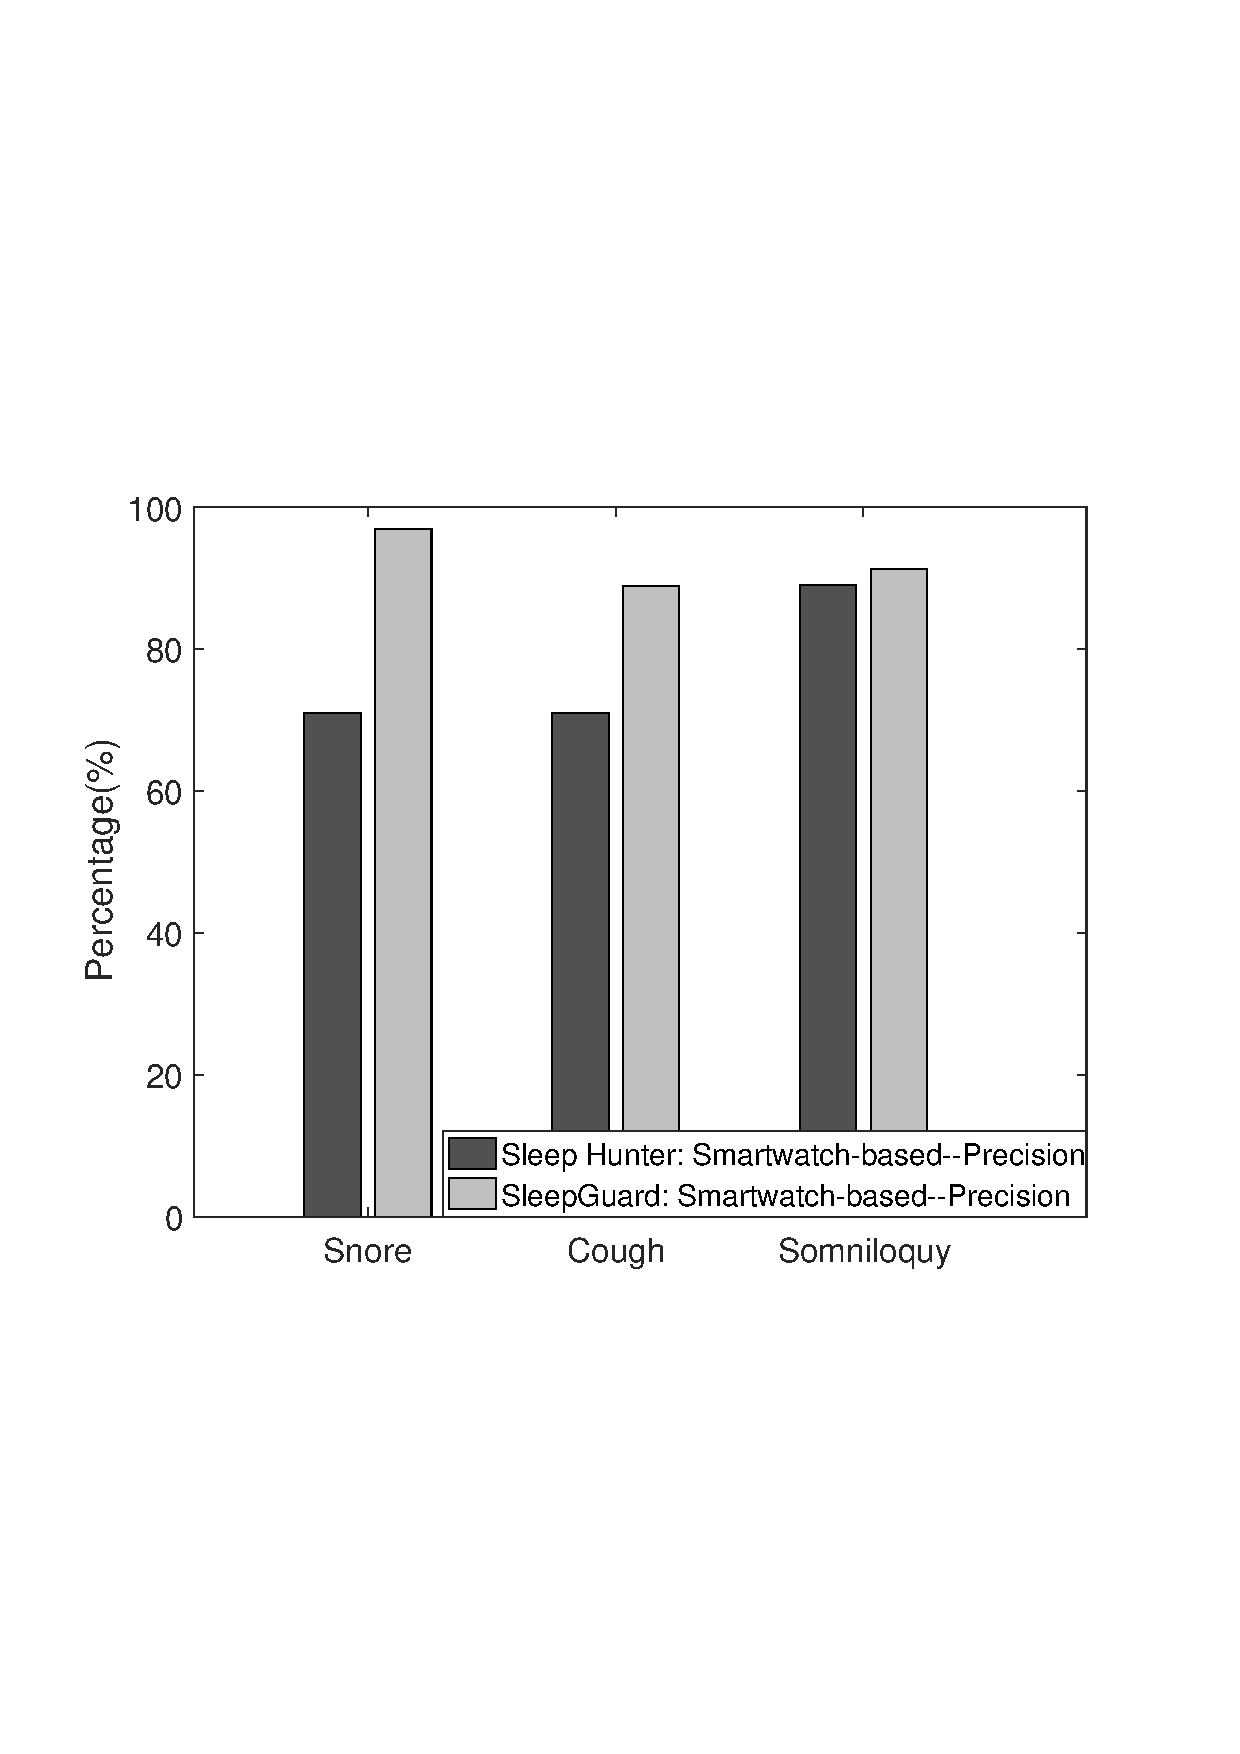
\includegraphics[width=0.45\linewidth]{Figures/compare_sound21.pdf}}
	\subfigure[Recall]{\label{compare_reca}
		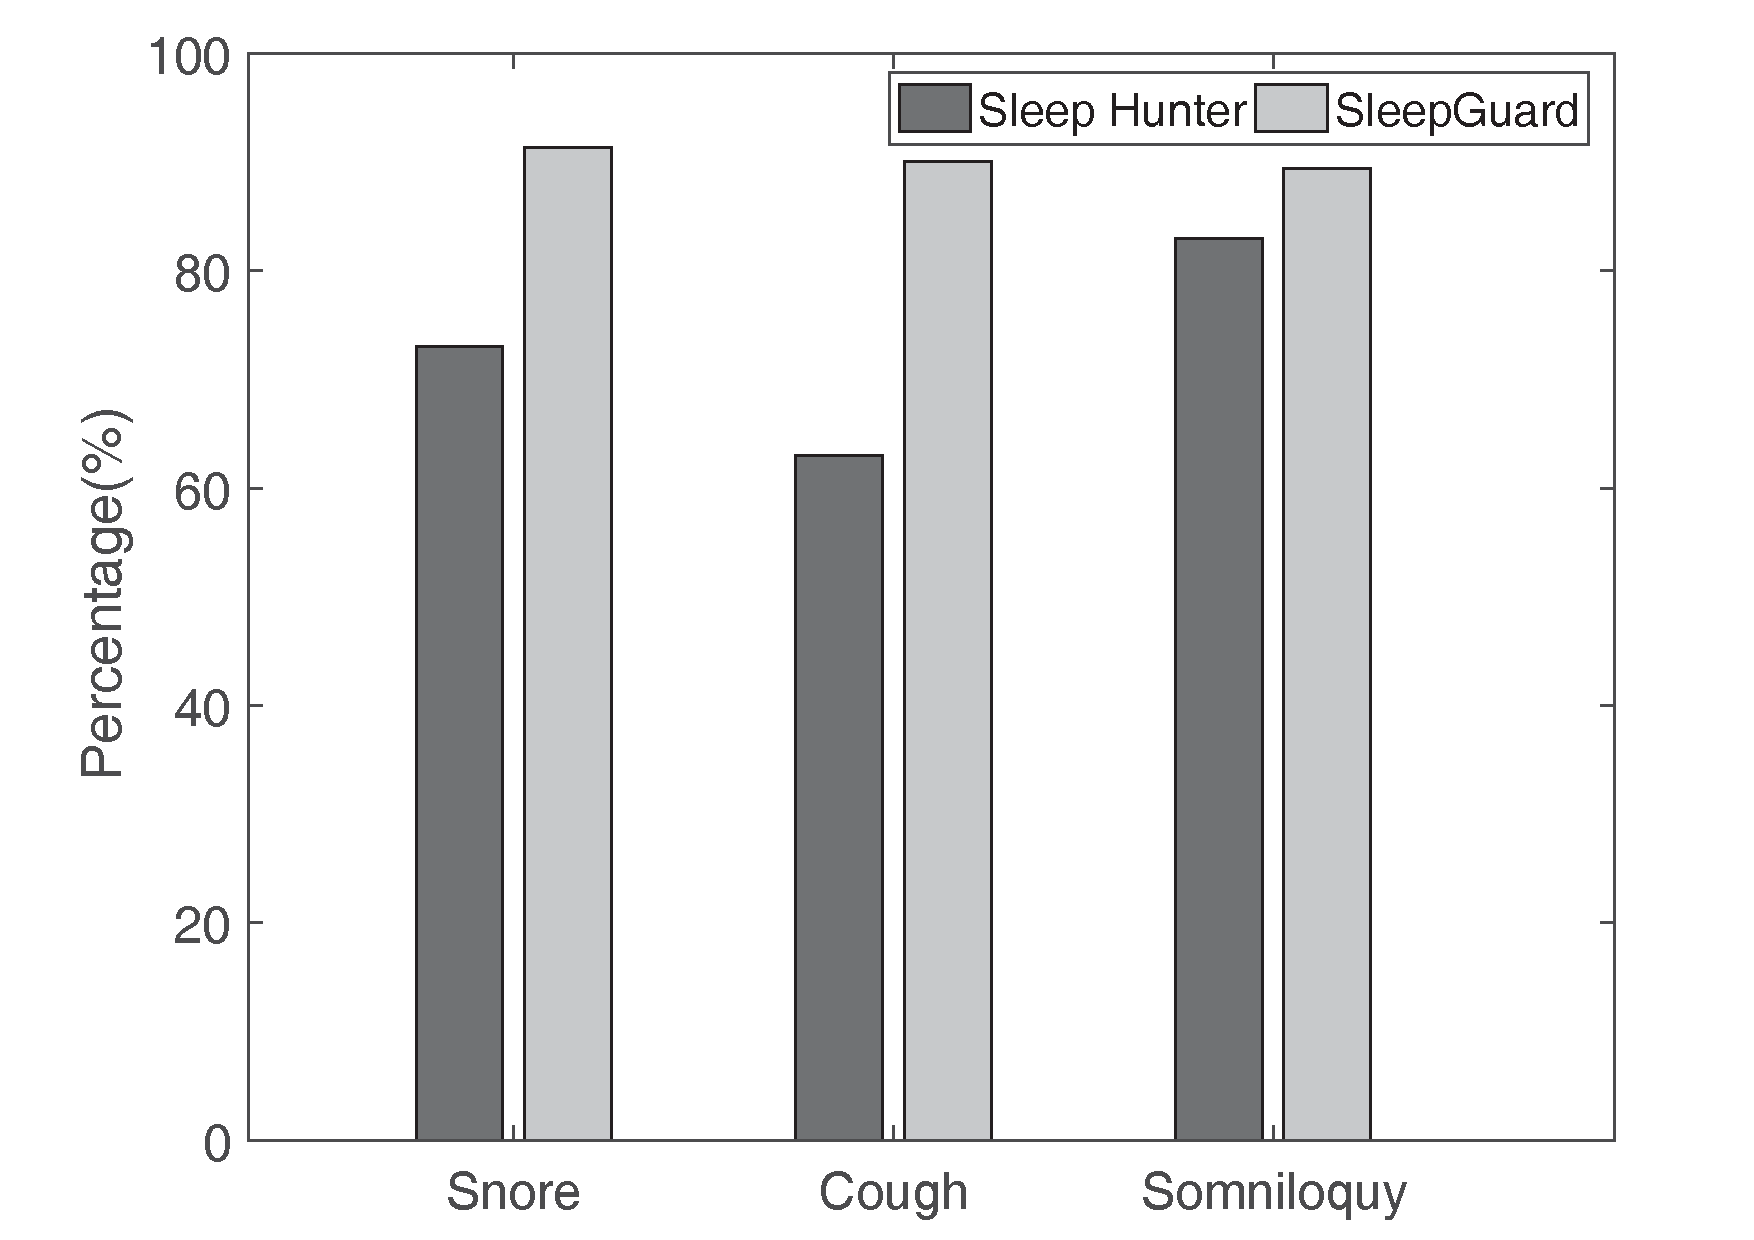
\includegraphics[width=0.45\linewidth]{Figures/compare_sound22.pdf}}
	\caption{Applying the event detection algorithms in Sleep Hunter our smartwatch data and compare them with \systemname.}\label{fig:compare_sound1}
\end{figure}

\begin{figure}[!t]
	\centering
    	\subfigure[Precision]{\label{compare_prec}
		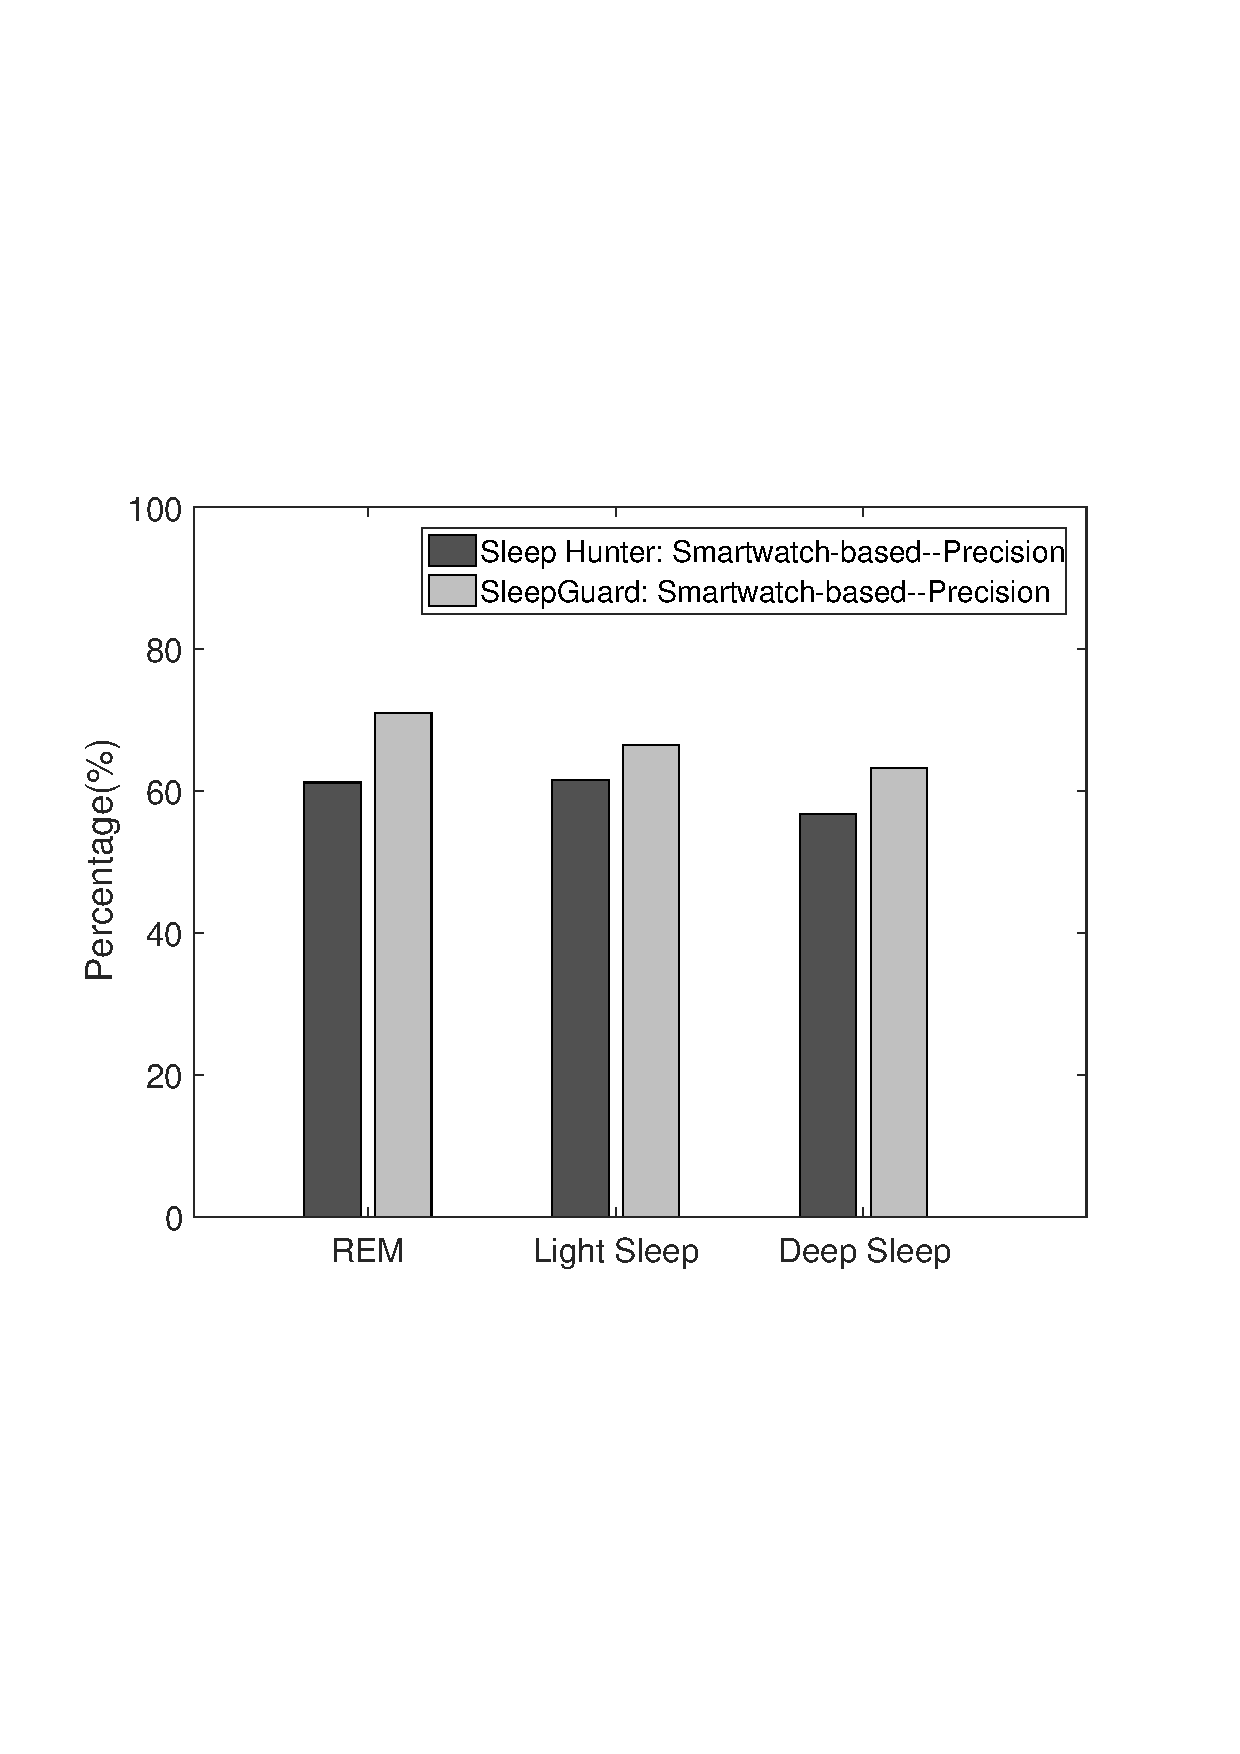
\includegraphics[width=0.45\linewidth]{Figures/compare_stage21.pdf}}
	\subfigure[Recall]{\label{compare_reca}
		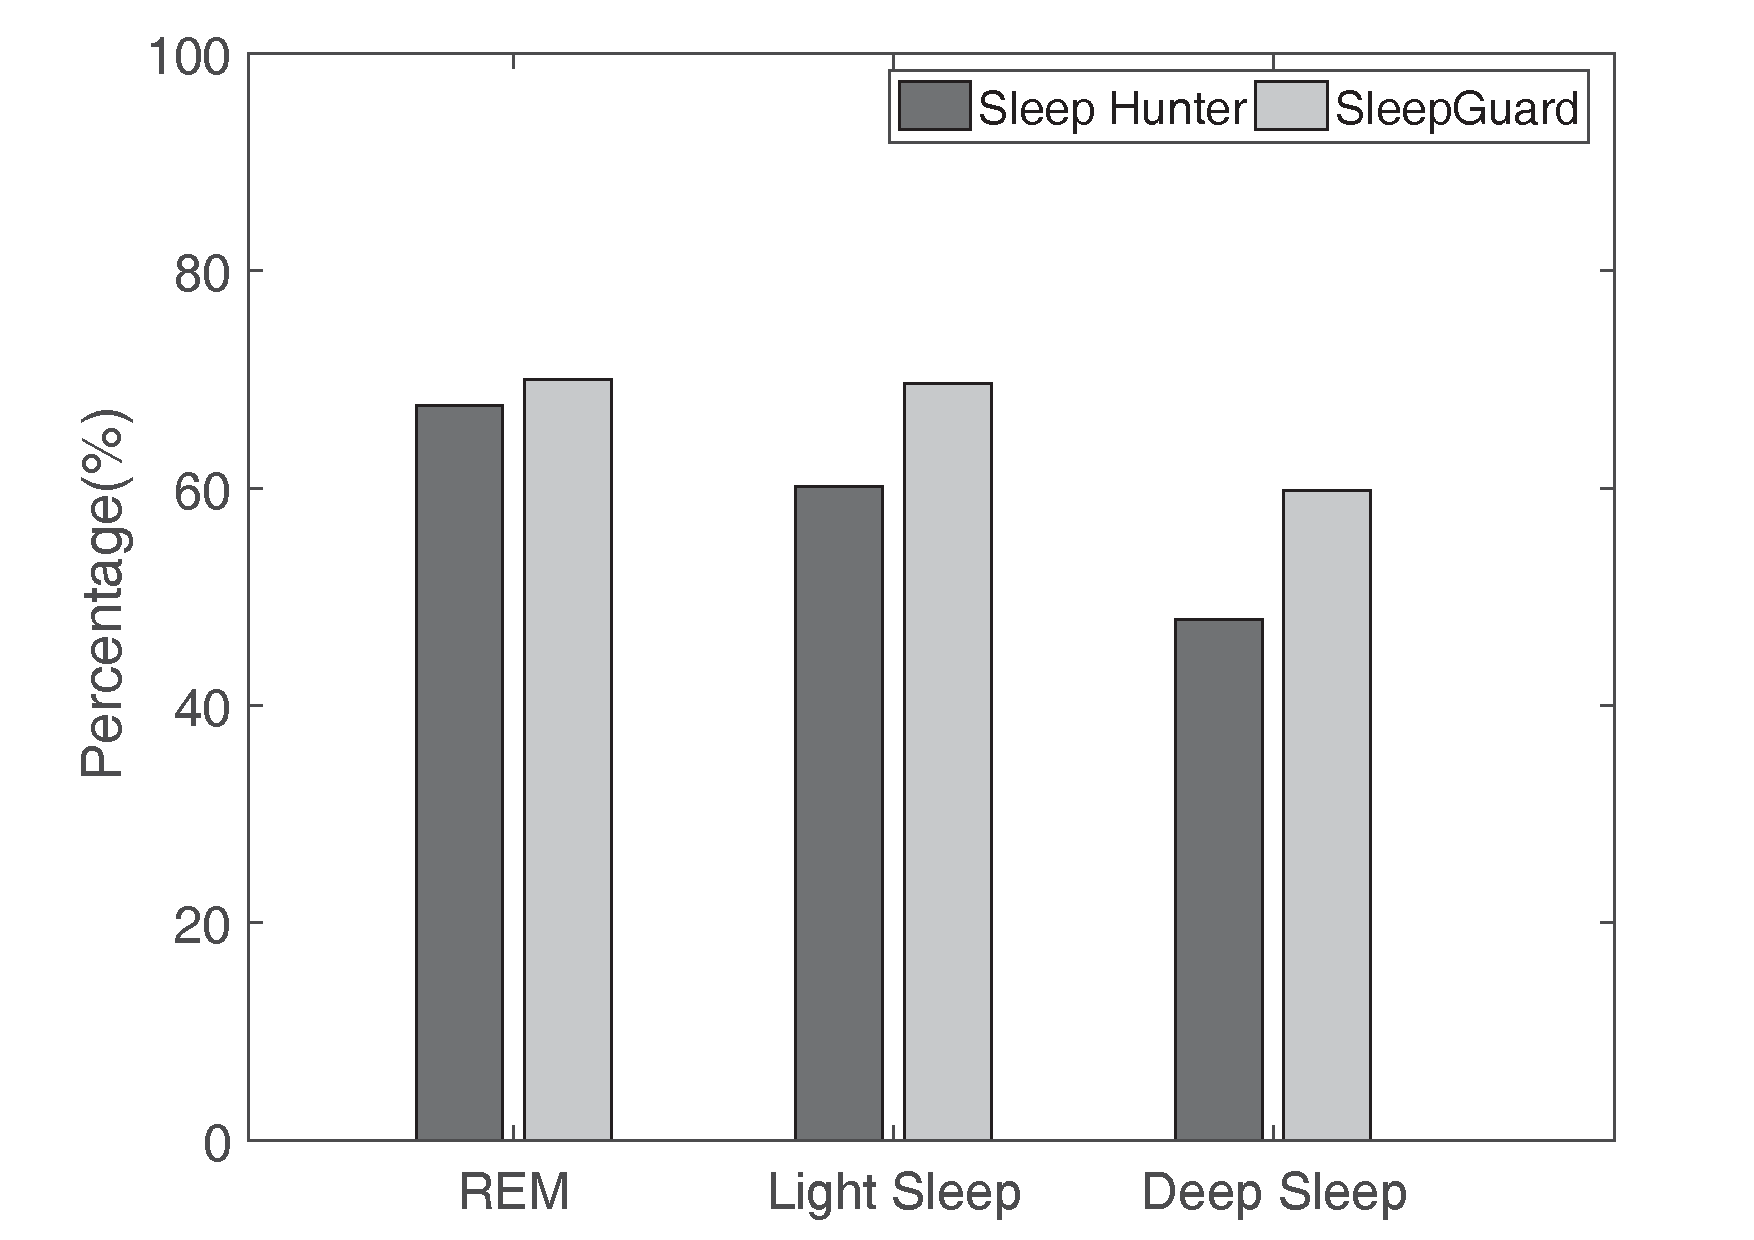
\includegraphics[width=0.45\linewidth]{Figures/compare_stage22.pdf}}
	\caption{Aplying the sleep stage detection algorithms in Sleep Hunter to our smartwatch  data and compare them with \systemname.}\label{fig:compare_stage1}
\end{figure}
%\begin{figure}[t!]
%	\centering
%	\begin{minipage}{.49\textwidth}
%\centering
%		 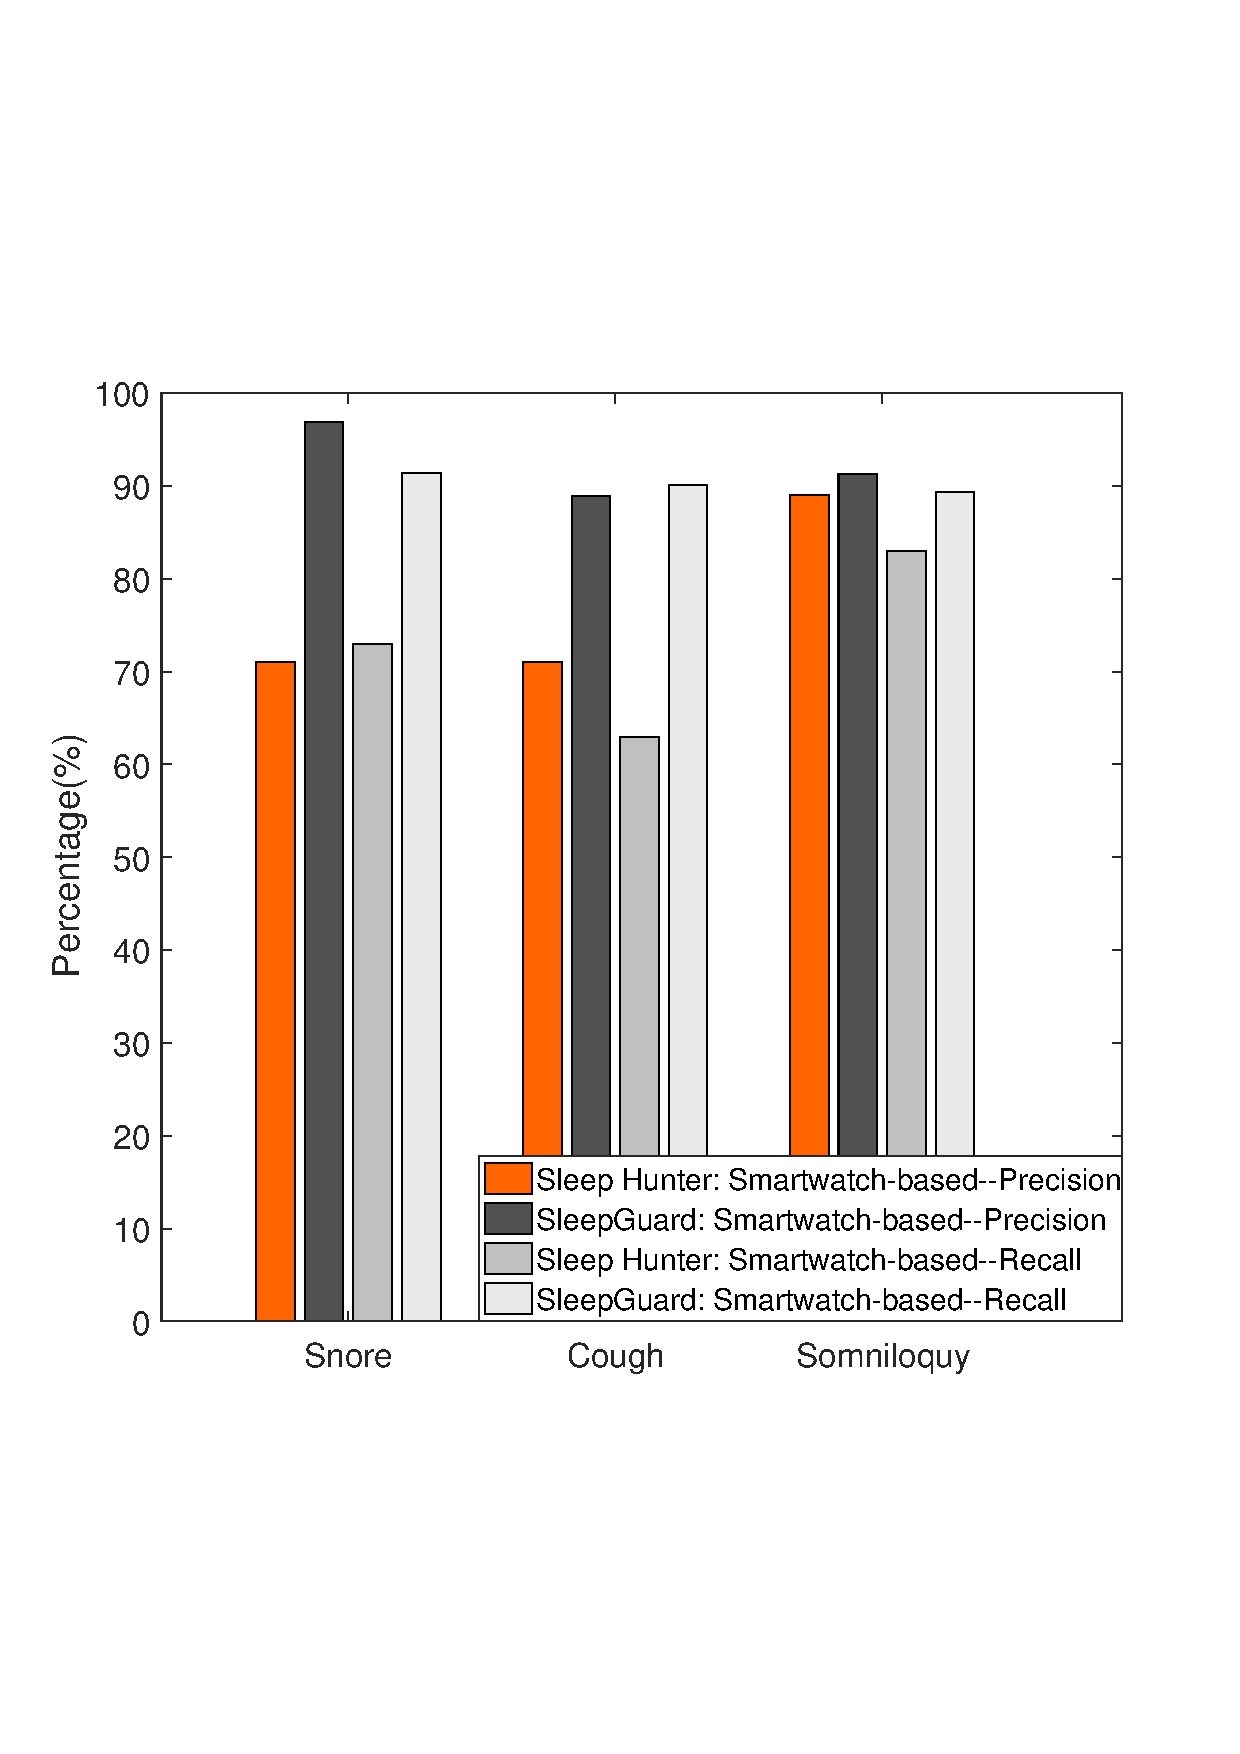
\includegraphics[width=5.7cm,height=4.7cm]{Figures/compare_sound1.pdf}
 % \caption{Applying the event detection algorithms in Sleep Hunter our smartwatch data and compare them with SleepGuard.}\label{fig:compare_sound1}
	%\end{minipage}%
%\hspace{2pt}
%	\begin{minipage}{.49\textwidth}
%	 \centering
%	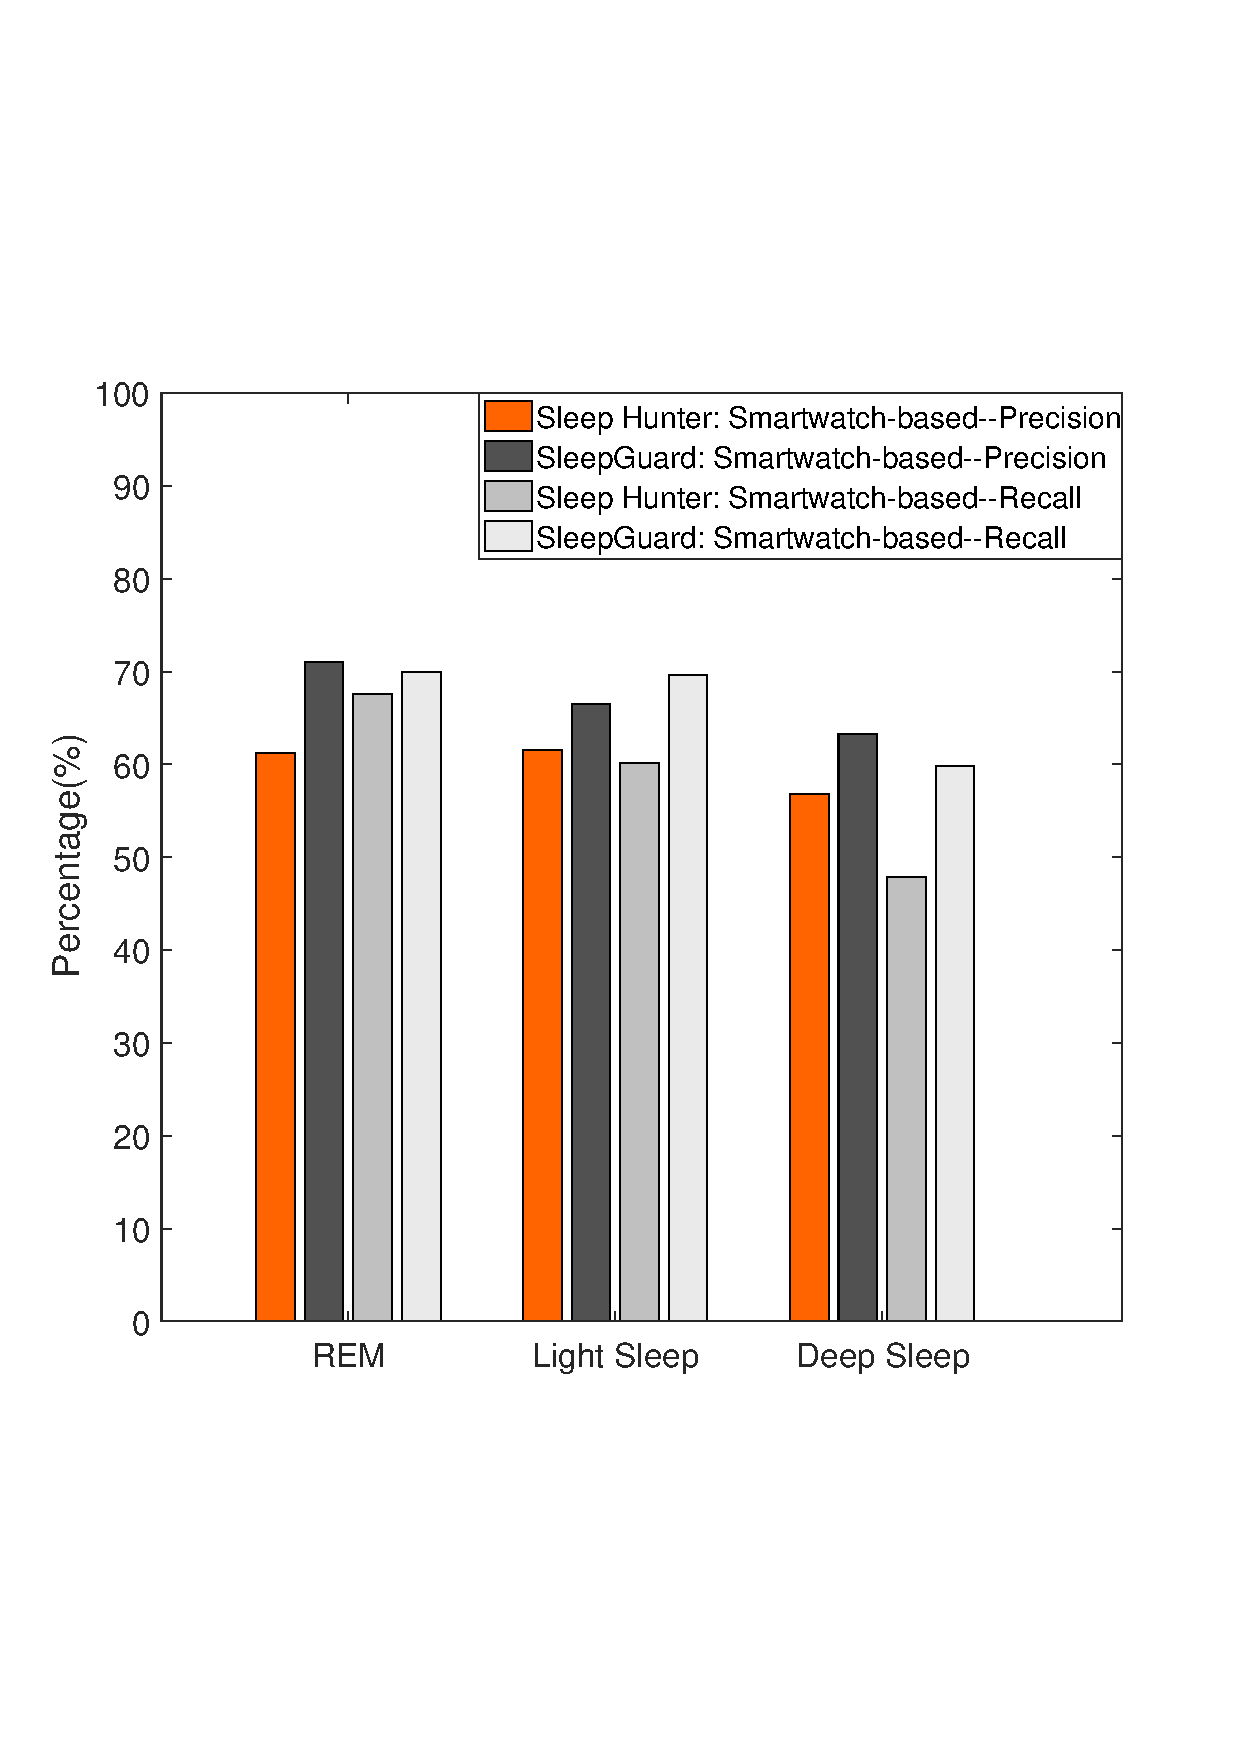
\includegraphics[width=5.7cm,height=4.7cm]{Figures/compare_stage1.pdf}
 % \caption{Aplying the sleep stage detection algorithms in Sleep Hunter to our smartwatch  data and compare them with SleepGuard.}\label{fig:compare_stage1}
%	\end{minipage}
%\end{figure}

\rt{We also implement the algorithms employed by Sleep Hunter, a smartphone-based solution, and apply them to the data collected using our
smartwatches. This experiment allows us to check if the better performance of \systemname is due to the use of a smartwatch instead of a
mobile phone.}

\rt{ For body movement detection, applying the algorithms employed by Sleep Hunter to our smartwatch data gives a comparable accuracy of
around 96\% when the system only identify between drastic and small body movements. However, Sleep Hunter doesn't work when we need to detect finer-grained body movements. %the accuracy of the Sleep Hunter
%algorithms drops to 78\% when we need to detect finer-grained body movements.
 \systemname outperforms Sleep Hunter by delivering an accuracy of drastic body movements around 90\% (see Table~\ref{tab:rollver}) and an accuracy of finer-grained body movements more than 78\% (see Fig.~\ref{fig:micro_combine}). For acoustic event detections, we apply
the Sleep Hunter algorithms to detect snore, cough and somniloquy. The results in Fig.~\ref{fig:compare_sound1} suggest that \systemname
gives better performance over Sleep Hunter in detecting these acoustic events. Finally, we apply the sleep stage detection model used by
Sleep Hunter to combine sleep-related events to identify sleep stages. The results are shown in Fig.~\ref{fig:compare_stage1}. Again,
\systemname outperforms the Sleep Hunter model with a higher accuracy and recall. }


\rt{ This experiment confirms that the algorithms used by Sleep Hunter for sleep event and stage detection are not tuned for smartwatches.
Compared to Sleep Hunter, \systemname can detect sleep events and stages with a higher accuracy using a set of carefully designed methods
to target smartwatches. }

%\textcolor{red}{What's more, to better demonstrate the advancement of our algorithm itself, not the benefits of equipment changes, we
%reproduce some algorithms of Sleep Hunter and apply its algorithm to the sleep data collected by our smartwatch. For the algorithm of body
%movement detection, since the algorithm in Sleep Hunter can only perform two classifications, namely large body movement and tiny movement,
%we combine body rollover and arm raising that are originally marked in our data into large body movement, while regard the remaining two
%kind of micro-body movement as tiny movement, according to the definition in Sleep Hunter. And the results show that the accuracy of body
%motion detection is about 96\%, which is comparable to the results of using smartphone data in Sleep Hunter. Compared to \systemname,
%although this result seems to be better than our results, when we consider a more fine-grained event classification, the worst performance
%can still reach more than 78\%. For the detection of acoustic event, we only compare the results of the three types of events: snore,
%cough, and somniloquy. This is because the sound data in our smartwatch failed to detect the respiration event, which may be because in
%Sleep Hunter, the smartphone is placed on the pillow near the nose, making it sensitive to the sound of respiration,so that apneustic and
%tachypneic can be detected. Fig.~\ref{fig:compare_sound1} shows the results of the comparison. We can see that the results of applying the
%algorithm in Sleep Hunter to the smartwatch data are not better than \systemname. So it can show the advantages of our acoustic detection
%algorithm and this is not brought about by smartwatch. In particular, since the proximity sensor used in the illumination condition
%detection algorithm in Sleep Hunter is not available in the sensor of smartwatch, this algorithm is not compared. And we also use CRF model
%given by Sleep Hunter to combine these events to detect sleep stage detection. We can see the comprehensive performance comparison results
%form Fig.~\ref{fig:compare_stage1}. We find that the performance of smartwatch-based is worse than the performance of \systemname. So it
%can be seen that \systemname can achieve better performance than sleep Hunter on some algorithms and detect finer-grained events, and this
%is not only because of the use of smartwatch. Even though \systemname's performance in sleep stage detection is not much better than Sleep
%Hunter, we put more effort into help users better analyze the factors that affect sleep quality.}





\subsubsection{User Survey}
\label{sec:user_survey}

To understand and verify how the additional information captured by \systemname supports users, at the end of the experiments the participants were administrated a survey to the participants asking about their experiences with \systemname and their personal sleeping patterns. We combine these results with the subjective sleep quality estimates obtained through the PSQI questionnaires administered during the study. We considered two groups of users in our survey. As the main source of information we consider the $15$ participants of our experiments who were asked about their experiences with \systemname, their subjective sleep quality assessment, and details of their personal sleep patterns. This set of users was augmented with external participants who were asked about their interested in the events that \systemname is capable of detecting.  The questions in our survey include:
\begin{enumerate}
  \item Subjective sleep quality (5-levels, 1 for excellent and 5 for worst),
  \item Sleep duration,
  \item Sleep disturbances,
  \item Daytime dysfunction.
\end{enumerate}
For the above four items, each one is rated on a 1 to 5 scale. These scores are first summed to yield a total score, which ranges from 0 to 20. Then we merge every five neighbouring scores into one scale and eventually divide the total scores into four levels, recorded as 0, 1, 2 and 3, representing poor, general, good and excellent, respectively. This step is necessary to compare the results of the user survey against the sleep quality estimation provided by \systemname and Fitbit.

%The final sleep quality score comes from the comprehensive scores of above four questionnaires.

In Table \ref{tab:quality}, we show the mean sleep quality score across 14 days given by each user together the estimations produced by
\systemname and Fitbit. \rt{We also give the standard deviation of the scores across the 14-day period per user. This number is given in
the brackets next to the mean score.} \rt{The last two rows in Table~\ref{tab:quality} compare the estimation given by \systemname and
Fitbit against the user self-rating score. In these two specific rows, a label of `P' indicates an estimated score perfectly matches the
user score, a label of `O' means the estimation error is within one scale point (for example, \systemname rates the user sleep to be
excellent while the user's self-rating is good), and a label of `B' indicates the estimation error is greater than a scale point. As can be
seen from the table, the estimation given by \systemname is more likely to match the user's self-rating compared to Fitbit (as indicating
by having more `P' labels - 9 vs 6 ) and, unlike Fitbit, the estimation error given by \systemname is never greater than one scale point.
To further validate this, we calculated the Spearman $\rho$-correlation~\cite{richardson2015nonparametric} between the user scores and each
of the two systems, \systemname and Fitbit. \systemname provides higher correlation coefficient ($\rho = 0.842$) than Fitbit ($\rho =
0.500$). The difference in correlation was found statistically significant using an one-tailed test carried out through a Fisher r-z
transformation ($Z = 1.66, p < 0.05$).  In summary, \systemname thus gives a better sleep quality assessment compared to Fitbit in our
evaluation.}

While the results above demonstrate that \systemname is capable of accurately estimating sleep quality, the main benefit from \systemname
compared to previous works is not its sleep quality performance but its capability to analyse and capture the {\em root cause} of sleep
issues. To demonstrate this, we carried out a follow up analysis where we examined the events captured by \systemname for each of the six
users assessing their sleep quality negatively (poor or general subjective quality, i.e., rating 0 or 1 in Table~\ref{tab:quality}). For
four of the six users we were able to find clear causes for their poor sleep. For one of the users, \systemname indicated difficulties in
falling asleep, which was reflected in a high body rollover count. Further analysis of captured events indicated ambient noise and lighting
to be most likely reasons for this participant. Another user complained feeling of numbness in the arm after sleep. Events captured by
\systemname showed that this was likely due to bad hand posture as the person tended to put the hand on top of head before sleeping. Third
user complained of frequent nightmares. Analysis of \systemname events showed that the person habitually slept on the left side, which has
been shown to have higher risk on nightmares~\cite{nightmare}, and often placed a hand on top of the chest, which creates additional
pressure and can lead to nightmares. Finally, one of the users mentioned suffering from long-term snoring problems, which we also were able
to detect from the events captured by \systemname. The events also highlighted that the person was often sleeping in supine position, which
further increases susceptibility to snoring-related problems. Existing systems are only capable of capturing some of these factors
influencing sleep quality and thus they are not capable of providing a holistic view of the participant's sleep quality, whereas
\systemname is capable of providing very detailed information about sleep events. To further demonstrate the benefits of \systemname
compared to previous works, we asked the 15 participants to make appropriate adjustments according to our recommendations and to conduct a
return visit survey three weeks later. It was found that some of the users were able to reduce symptoms and to improve their average
quality of sleep based on the suggestions.

		
	%For one user, the light intensity and ambient noise detection indicated frequent light and noise pollution, and hence is most likely cause of poor sleep. This fin
	
%		Through {\systemname}'s detecting, one user showed obvious symptoms of the difficulty of falling asleep and an unusually high number of body rollover. Our further analysis revealed that there was excessive light intensity and frequent noise in his sleeping environment. This may have led to the appearance of these symptoms and thus the poor quality of sleep.
	%we summarized the sleep problems and habit of the 15 volunteers who participated in our system assessment through a questionnaire survey and quality of sleep assessment. Then we found that there is a participant reported that his arm was always paralyzed, and five participants had poor sleep quality. We can find that the reason why the user's arm is numb is his incorrect sleep habits. The results from {\systemname} showed that he always tends to put his hands on his head, and long-term postures like this will inevitably lead to numbness of the arms. For similar situations, we will inform and remind users of their inappropriate postures and habits, and recommend that users should take measures to improve such situations.
	


%And there is a user reported that he always had a nightmare at night, which led to poor sleep quality. We analyse the results of {\systemname} and found that user has been accustomed to sleep in the left side, and sometimes the hand is habitually placed on the chest. As \cite{nightmare} points that people who sleep on their left side are more at risk of nightmares. And the oppression of the chest by the hand causes the brain to have an ill hallucination, making it extremely easy to make a nightmare. So {\systemname} suggest to the user based on these two possible reasons, and hope that the user can take some special measures to change it, and recommend that the user can take some additional methods, such as listening to some soothing music to relax before sleep. Another user was detected by {\systemname} to be bothered by long-term snoring, as he himself mentioned. We know that the occurrence of snoring is most likely due to improper sleeping posture, and we also detected that the user is accustomed to sleep in a supine position, so on the one hand, {\systemname} suggests that the user try the sleeping position in the side position. On the other hand, if the situation still does not improve very well, it is recommended that the user go to the hospital in time for a corresponding check to avoid snoring caused by certain diseases. In addition, if we detect that some users are accustomed to sleeping in a prone position, we will remind and advise them because the prone position is bad for health.}

%\textcolor{blue}{According to different possible reasons, {\systemname} proposes different reminders and suggestions to users, such as adjusting their sleeping posture, improving the sleeping environment, and consciously avoiding bad sleeping habits. As for how to adjust and avoid them, users can take special, mandatory or medical methods according to their own situation. FAnd it }
	
As for the user experience, results from the survey highlighted a strong interest in the information captured by \systemname. In particular, 80\% of participants believe that the detection of sleep posture is very necessary, showing their sleep posture can not only help people to avoid health problems caused by long-term improper sleeping posture, but also help us find out the reasons for the next day's physical discomfort, such as dizziness, muscle soreness may be due to improper sleeping posture. And there are some users are troubled by snoring. This may be due to improper sleeping posture. We map the detected snoring event and sleeping posture to suggest the user to modify his posture to a suitable posture to reduce the harm caused by long-term snoring. 60\% of the participants thought it useful to detect the hand position in supine posture, even one user mentioned that he did often have nightmares and our system found his hand was often placed on his chest, and then {\systemname} could remind him that he should take some measures to avoid such a position and thus reduce the poor sleep quality that nightmare brings. Only 20\% of participants found it useful to calculate the number of body rollover. However, detection of rollovers is useful in segmenting sleep stages. Furthermore, body rollover counts could be used to derive additional information to the user, such as how restless or peaceful the sleep has been overall.


\begin{table} \tiny%\scriptsize%\footnotesize
  \centering \caption{\rt{Results of sleep quality assessments. The first three rows show the sleep quality scores of the different systems
  (mean and standard deviation) for each user across $14$ days, whereas the last two rows  compare sleep quality labels between subjective
  assessments and those returned by \systemname and FitBit. }}\label{tab:quality}
\begin{tabularx}{\textwidth}{X cccccccccccccccc }
        \toprule
         \textbf{User ID} & 1 & 2 & 3 & 4 & 5 & 6 & 7 & 8 & 9 & 10 & 11 & 12 & 13 & 14 & 15\\
         \midrule
         \rowcolor{Gray}\systemname & 3 (1.8) & 3 (1.5) & 0 (1.0) & 1 (1.8) &  2 (1.2) &  2 (1.7) &  3 (1.0) & 0 (1.3) &  2 (1.3) &  2 (1.0) & 2 (0) & 2 (1.5) &  1 (1.8) &  0 (1.0) &  2 (1.3)\\
         Fitbit & 3 (1.7) & 3 (2.2) & 0 (1.3) & 0 (1.8) & 1 (2.2) & 3 (1.8) & 2 (1.9) & 3 (1.8) & 2 (1.7) & 2 (1.9) & 2 (1.3) & 2 (2.0) & 2 (2.3) & 1 (1.8) & 2 (1.7) \\
         \rowcolor{Gray} User score & 3 (0.0) & 2 (1.4) & 0 (0.0) &  0 (1.7) & 2 (1.7) &  2 (1.0) & 3 (1.0) & 1 (1.7) & 1 (1.4) & 2 (1.0) &  2 (1.0) & 3 (2.0) & 0 (1.8) & 0 (1.0) & 2 (1.0) \\
         User score matching (\systemname) & P&O&P&O&P&P&P&O&O&P&P&O&O&P&P\\
         \rowcolor{Gray} User score matching (Fitbit) & P&O&P&P&O&O&O&\textbf{B}&O&P&P&O&\textbf{B}&O&P     \\
         \bottomrule
\end{tabularx}
\end{table}


%\begin{table} \footnotesize
%  \centering  % ������
%  \renewcommand\arraystretch{0.5}
%  \caption{Results of sleep quality assessment.}\label{tab:quality}
%\begin{tabular}{|c| c | c | c | c | c |c |c |c |c |c| c |c |c |c |c |c }
%    \cline{1-16}
%    %\multicolumn{1}{c|}{\textbf{}}
%    %&
%      \multicolumn{1}{|c|}{\diagbox{System}{User ID}}
%    &  \multicolumn{1}{c|}{\footnotesize  1}
%    &  \multicolumn{1}{c|}{\footnotesize  2}
%    &  \multicolumn{1}{c|}{\footnotesize  3}
%    &  \multicolumn{1}{c|}{\footnotesize  4}
%    &  \multicolumn{1}{c|}{\footnotesize  5}
%    &  \multicolumn{1}{c|}{\footnotesize  6}
%    &  \multicolumn{1}{c|}{\footnotesize  7}
%    &  \multicolumn{1}{c|}{\footnotesize  8}
%    &  \multicolumn{1}{c|}{\footnotesize  9}
%    &  \multicolumn{1}{c|}{\footnotesize  10}
%    &  \multicolumn{1}{c|}{\footnotesize  11}
%    &  \multicolumn{1}{c|}{\footnotesize  12}
%    &  \multicolumn{1}{c|}{\footnotesize  13}
%    &  \multicolumn{1}{c|}{\footnotesize  14}
%    &  \multicolumn{1}{c|}{\footnotesize  15}\\
%     \cline{1-16}
%     & & & & & & & & & & & & & & & \\
%    \multirow{16}{*}
%      \textbf{\footnotesize {\systemname}}  & $3$ & $3$ & $0$ & $1$ & $2$ & $2$ & $3$ & $0$ & $2$ & $2$ & $2$ & $2$ & $1$ & $0$ & $2$ \\
%   & & & & & & & & & & & & & & & &\\
%    \cline{1-16}
%   & & & & & & & & & & & & & & & &\\
%     \textbf{\footnotesize Fitbit}   & $3$ & $3$ & $0$ & $0$ & $1$ & $3$ & $2$ & $3$ & $2$ & $2$ & $2$ & $2$ & $2$ & $1$ & $2$\\
%      & & & & & & & & & & & & & & & & \\
%      \cline{1-16}
%       & & & & & & & & & & & & & & & & \\
%      \textbf{\footnotesize User survey}  & $3$ & $2$ & $0$ & $0$ & $2$ & $2$ & $3$ & $1$ & $1$ & $2$ & $2$ & $3$ & $0$ & $0$ & $2$ \\
%     & & & & & & & & & & & & & & & & \\
%     \cline{1-16}
%      \cline{1-16} \rowcolor[RGB]{199,201,203}
%      & \multicolumn{1}{>{\columncolor[RGB]{112,113,116}}c|}{}& &\multicolumn{1}{>{\columncolor[RGB]{112,113,116}}c|}{} & & & & & &
%      & \multicolumn{1}{>{\columncolor[RGB]{112,113,116}}c|}{}
%      & \multicolumn{1}{>{\columncolor[RGB]{112,113,116}}c|}{}& & & &\multicolumn{1}{>{\columncolor[RGB]{112,113,116}}c|}{} \\ \rowcolor[RGB]{199,201,203}
%
%     \textbf{\footnotesize Compatibility}  & \multicolumn{1}{>{\columncolor[RGB]{112,113,116}}l|}{3} & $2$ &
%     \multicolumn{1}{>{\columncolor[RGB]{112,113,116}}c|}{3} & $2$ & $3$ & $3$ & $3$ & $2$ & $2$ &
%     \multicolumn{1}{>{\columncolor[RGB]{112,113,116}}c|}{3} & \multicolumn{1}{>{\columncolor[RGB]{112,113,116}}c|}{3} & $2$ & $2$ & $3$ &
%     \multicolumn{1}{>{\columncolor[RGB]{112,113,116}}c|}{3} \\ \rowcolor[RGB]{199,201,203}
%
%      & \multicolumn{1}{>{\columncolor[RGB]{112,113,116}}c|}{}& &\multicolumn{1}{>{\columncolor[RGB]{112,113,116}}c|}{} & & & & & &
%      & \multicolumn{1}{>{\columncolor[RGB]{112,113,116}}c|}{}
%      & \multicolumn{1}{>{\columncolor[RGB]{112,113,116}}c|}{}& & & &\multicolumn{1}{>{\columncolor[RGB]{112,113,116}}c|}{} \\ \rowcolor[RGB]{199,201,203}
%    \cline{1-16}
%   \end{tabular}
%\end{table}

%\begin{figure}
 %\centering
% 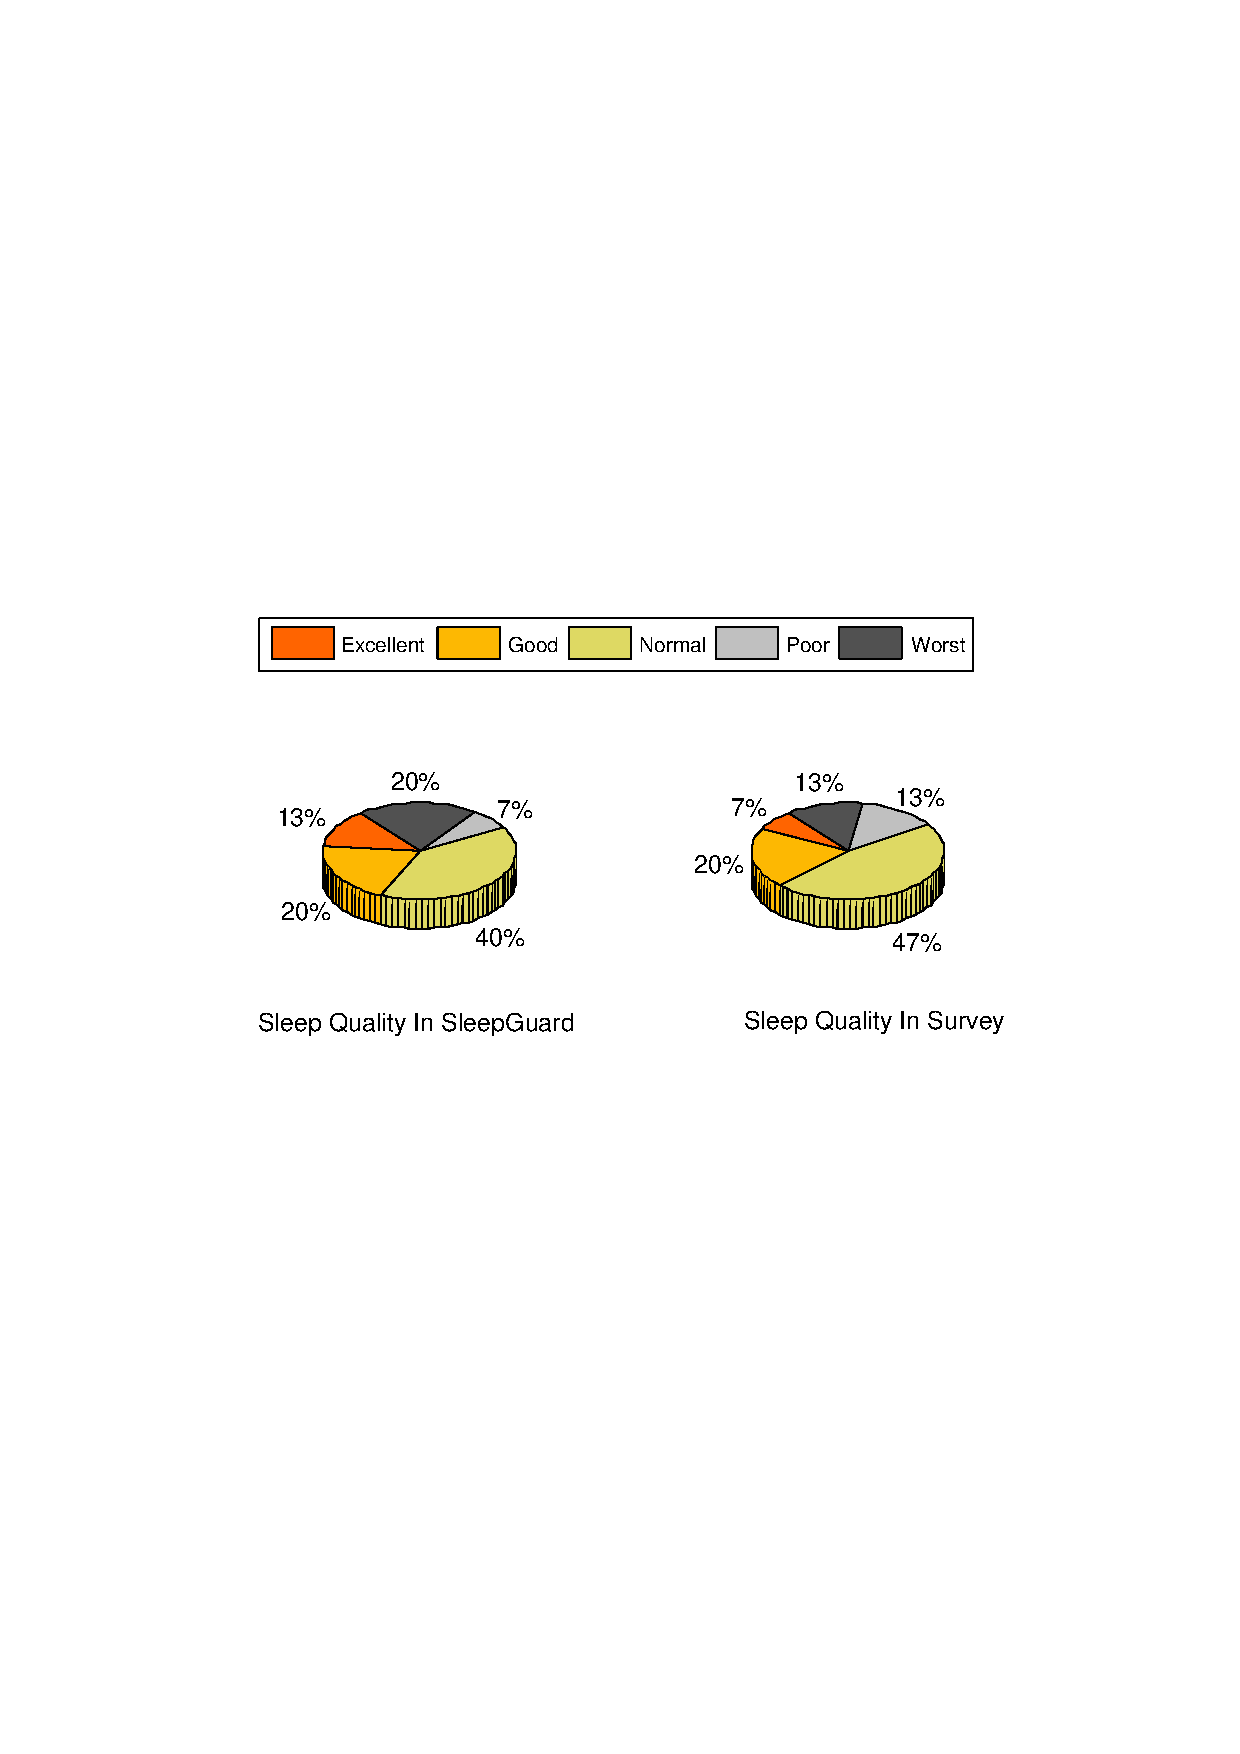
\includegraphics[width=0.52\linewidth]{Figures/quality.pdf}
 %\caption{Participants' sleep quality distribution}\label{fig:quality}
%\end{figure}
